% !TeX encoding = UTF-8
% !TeX root = V34_TEM.tex
% !TeX spellcheck = de_DE_frami

\section{Durchführung}

\subsection{Vorversuch optische Abbildungen}
Die Funktionsweise und Messmodi eines Elektronenmikroskops lassen sich anschaulich am Modell des Lichtmikroskops zeigen. Als Lichtquelle dient uns ein Laser, dessen Strahl durch eine Aufweitungsoptik aus zwei Linsen $L_1, L_2$ mit Brennweiten $f_1, f_2$ und Abstand $f_1 + f_2$ verbreitert wird. Dabei bündelt $L_1$ den Laserstrahl im Brennpunkt zwischen den Linsen, der als Punktquelle für $L_2$ dient und erneut parallelisiert wird. Gemäß dem Strahlensatz wird der Strahl dabei um den Faktor $\frac{f_2}{f_1}$ aufgeweitet, wodurch ein großer Bereich gleichmäßig ausgeleuchtet werden kann.

Nun werden verschiedene Objekte O durch zwei Linsen (Objektiv $L_3$, Okular $L_4$) auf die Wand $B$ abgebildet. Das Objektiv wird anschließend so verschoben, dass das Beugungsbild von O mit $g = \infty$ abgebildet wird.

\begin{figure}[h]
	\centering
	\def\svgwidth{0.75\textwidth}
	\input{graphics/light.pdf_tex}
	\caption{Zeichnung Lichtmikroskop, Abbildung des Objektes}
	\label{fig:Mikroskop}
\end{figure}


\subsubsection{Spalte und Gitter}
\enlargethispage{2\baselineskip}

\begin{figure}[p]
	\centering
	\begin{subfigure}[b]{0.49\textwidth}
		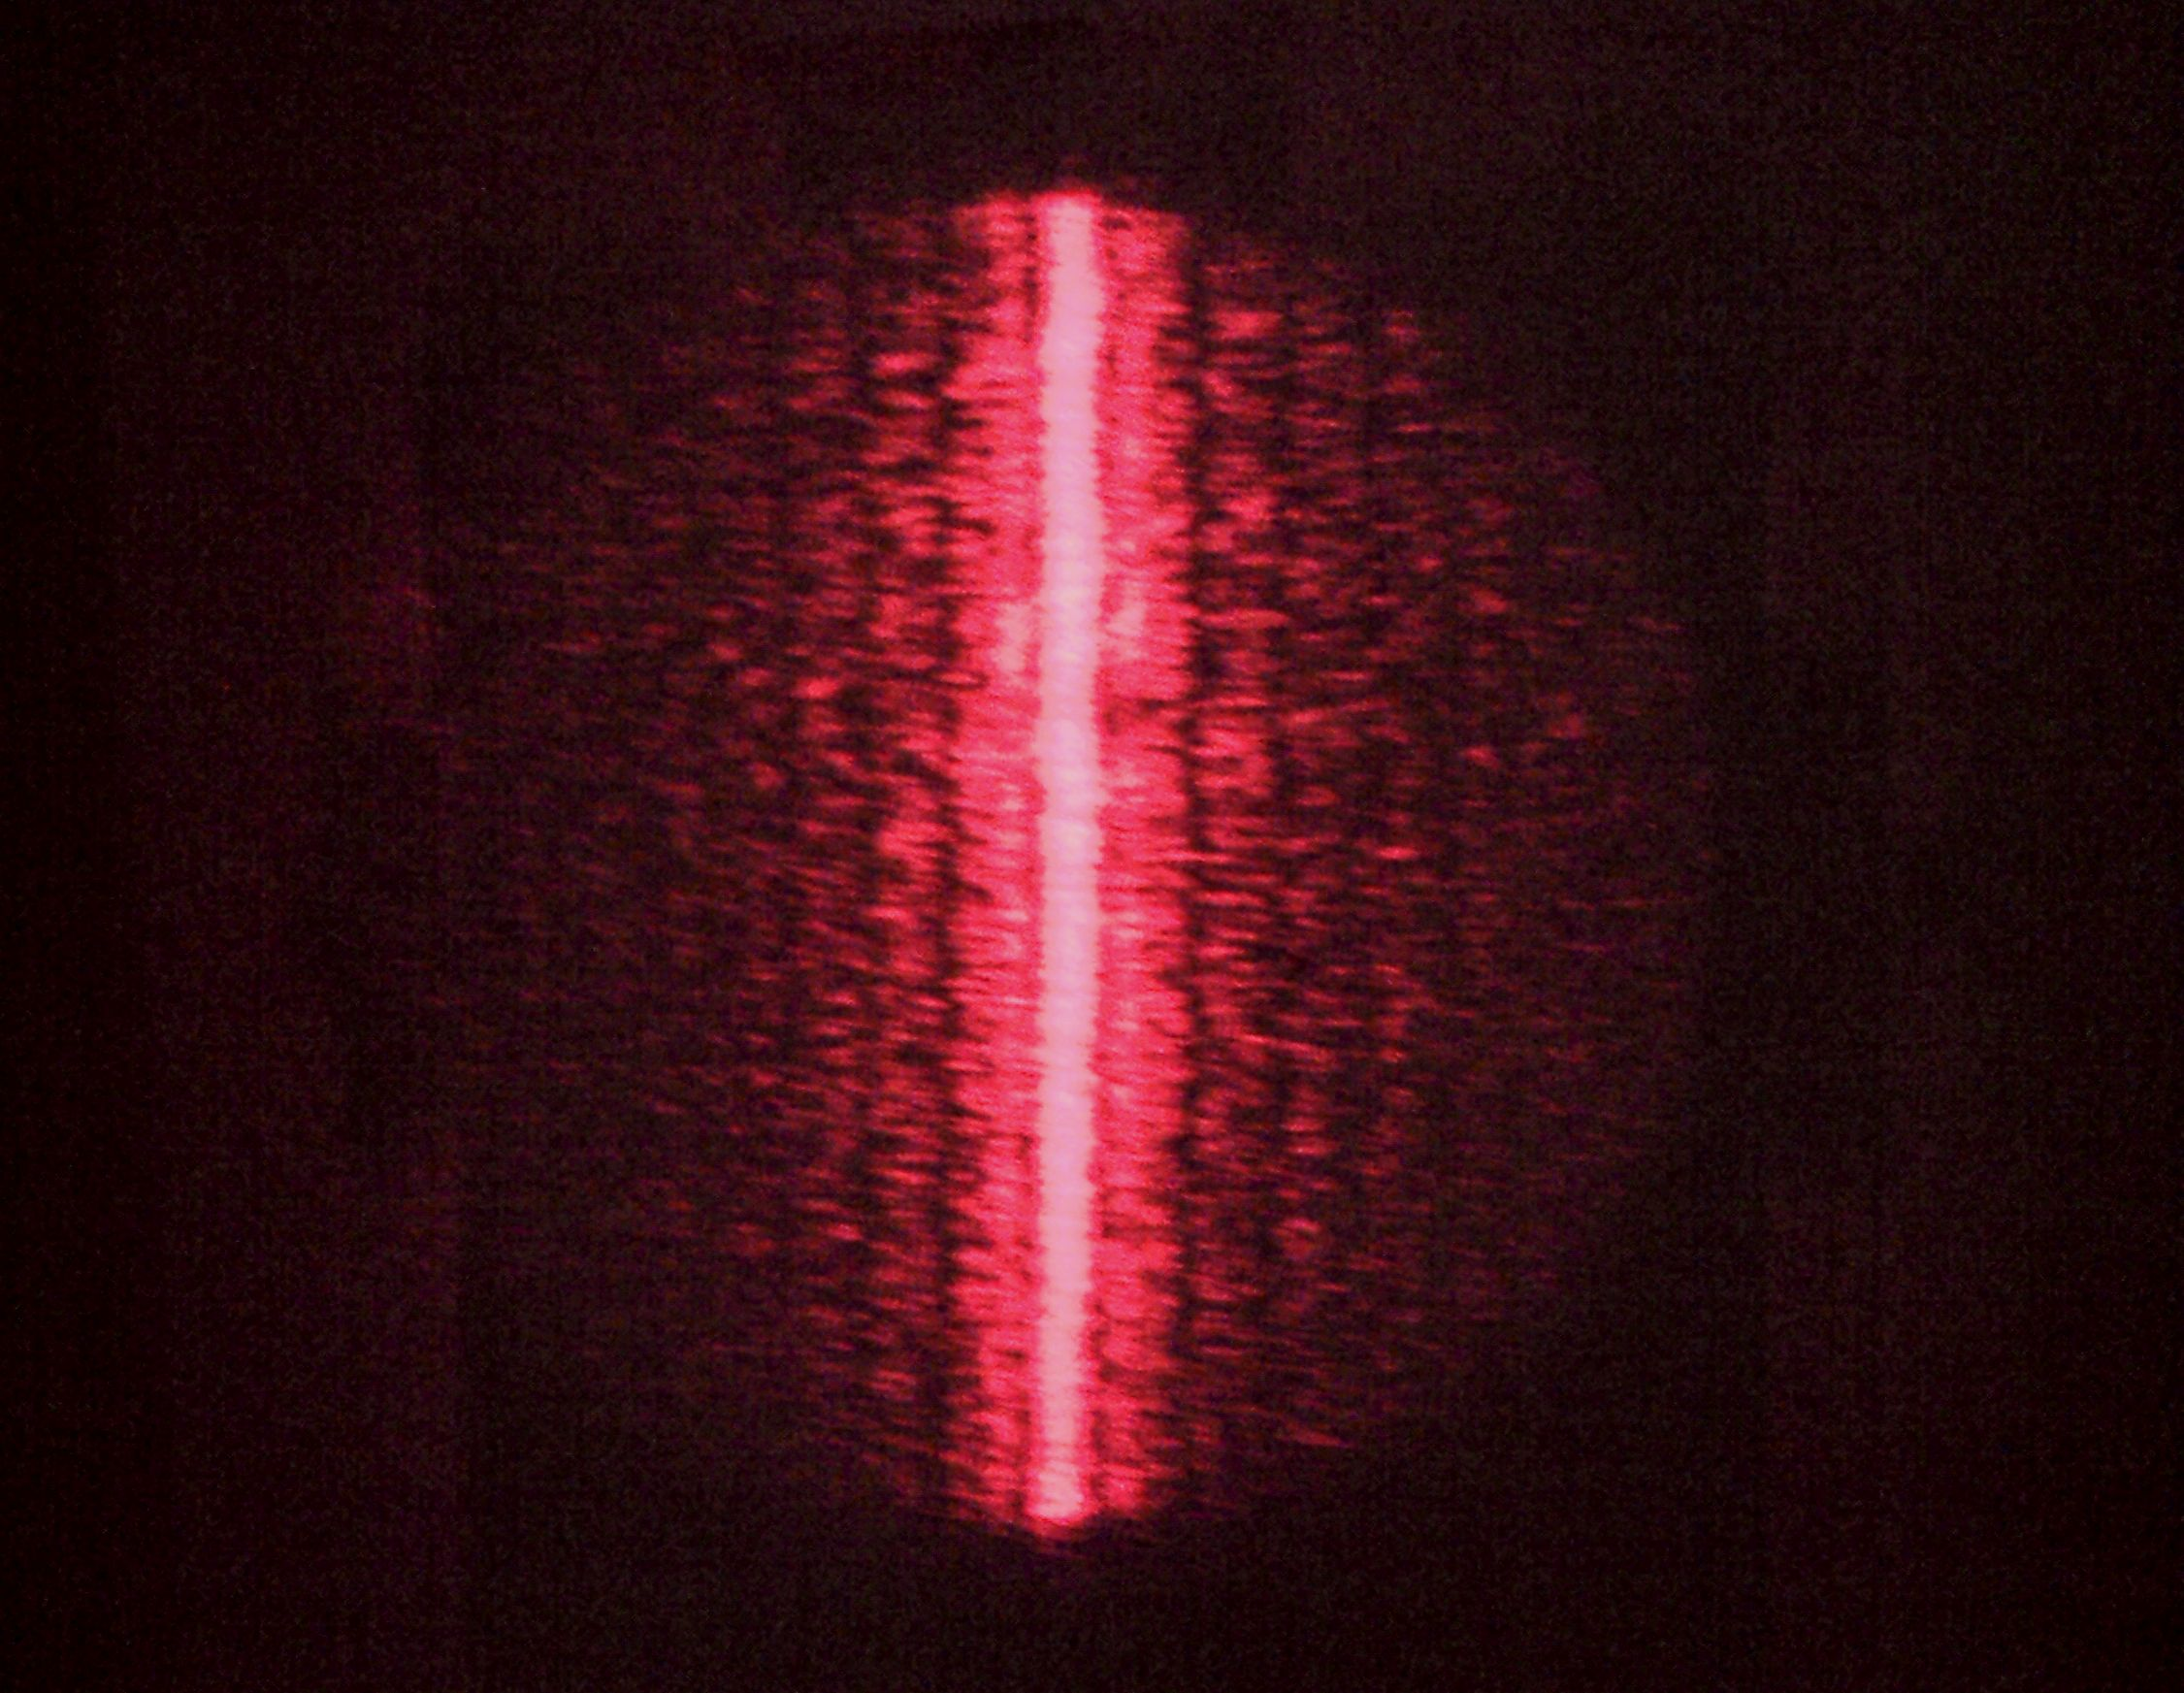
\includegraphics[width=\textwidth]{data/optics/02_Einzelspalt_Bild}
		\caption{Bild}
	\end{subfigure}
	\begin{subfigure}[b]{0.49\textwidth}
		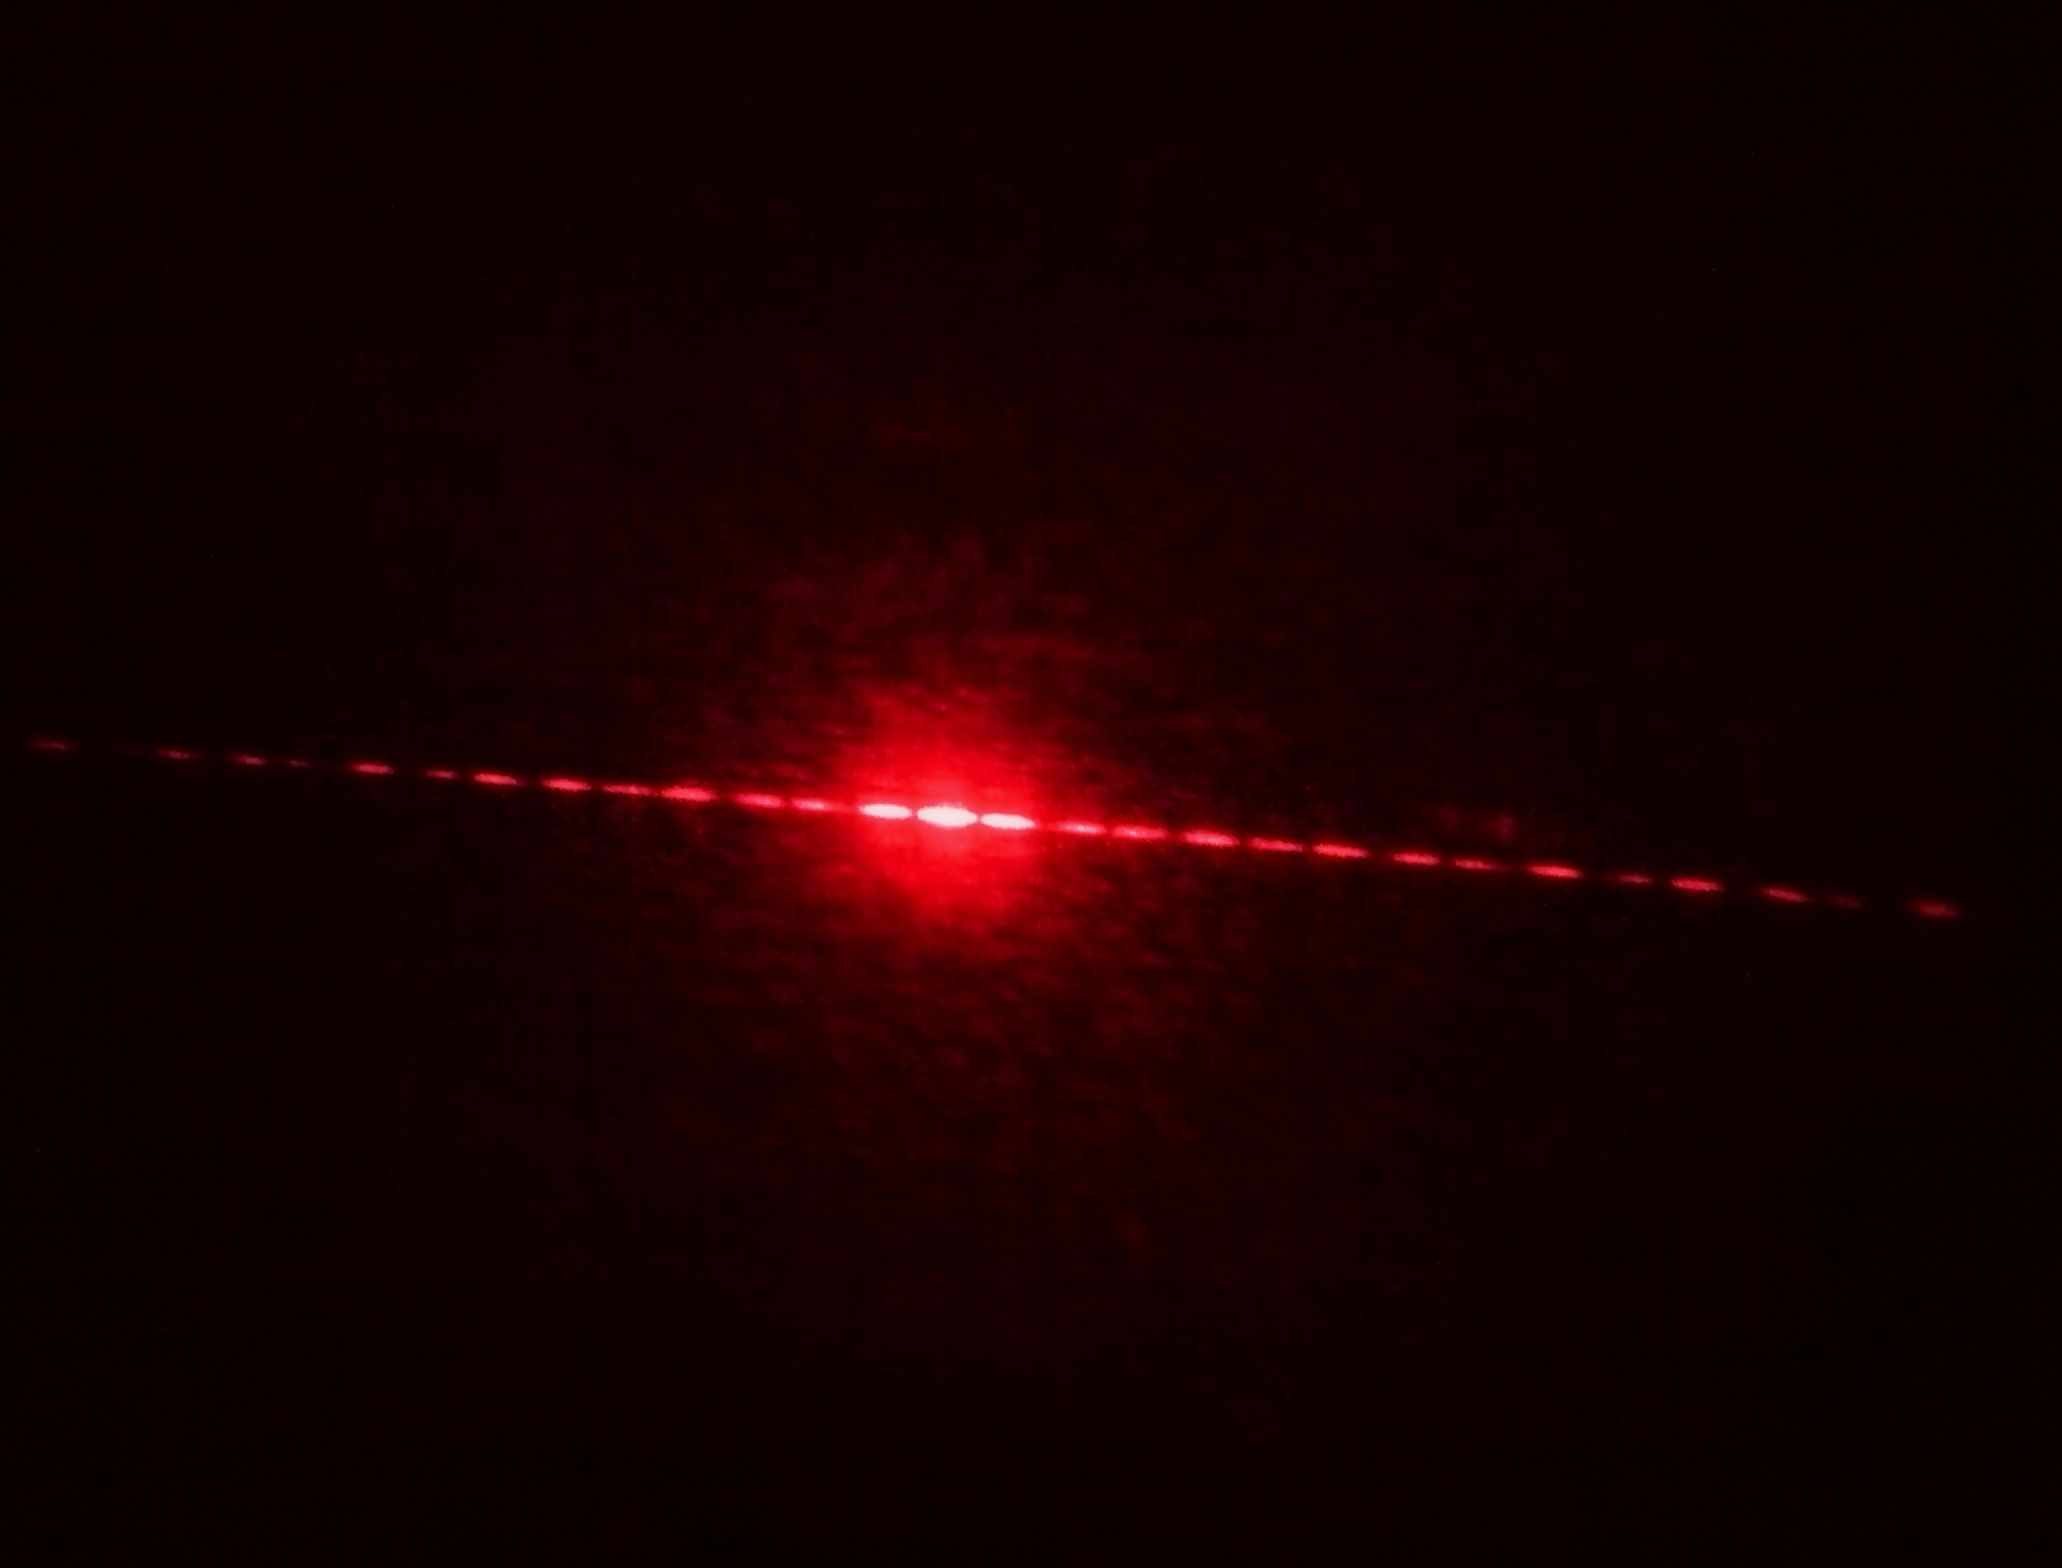
\includegraphics[width=\textwidth]{data/optics/02_Einzelspalt_Beugung}
		\caption{Beugungsbild} 		\label{fig:Einzel_BG}
	\end{subfigure}
	\caption{Einzelspalt}				\label{fig:Einzel}
	\vspace{-1em}
\end{figure}

\begin{figure}[p]
	\centering
	\begin{subfigure}{0.49\textwidth}
		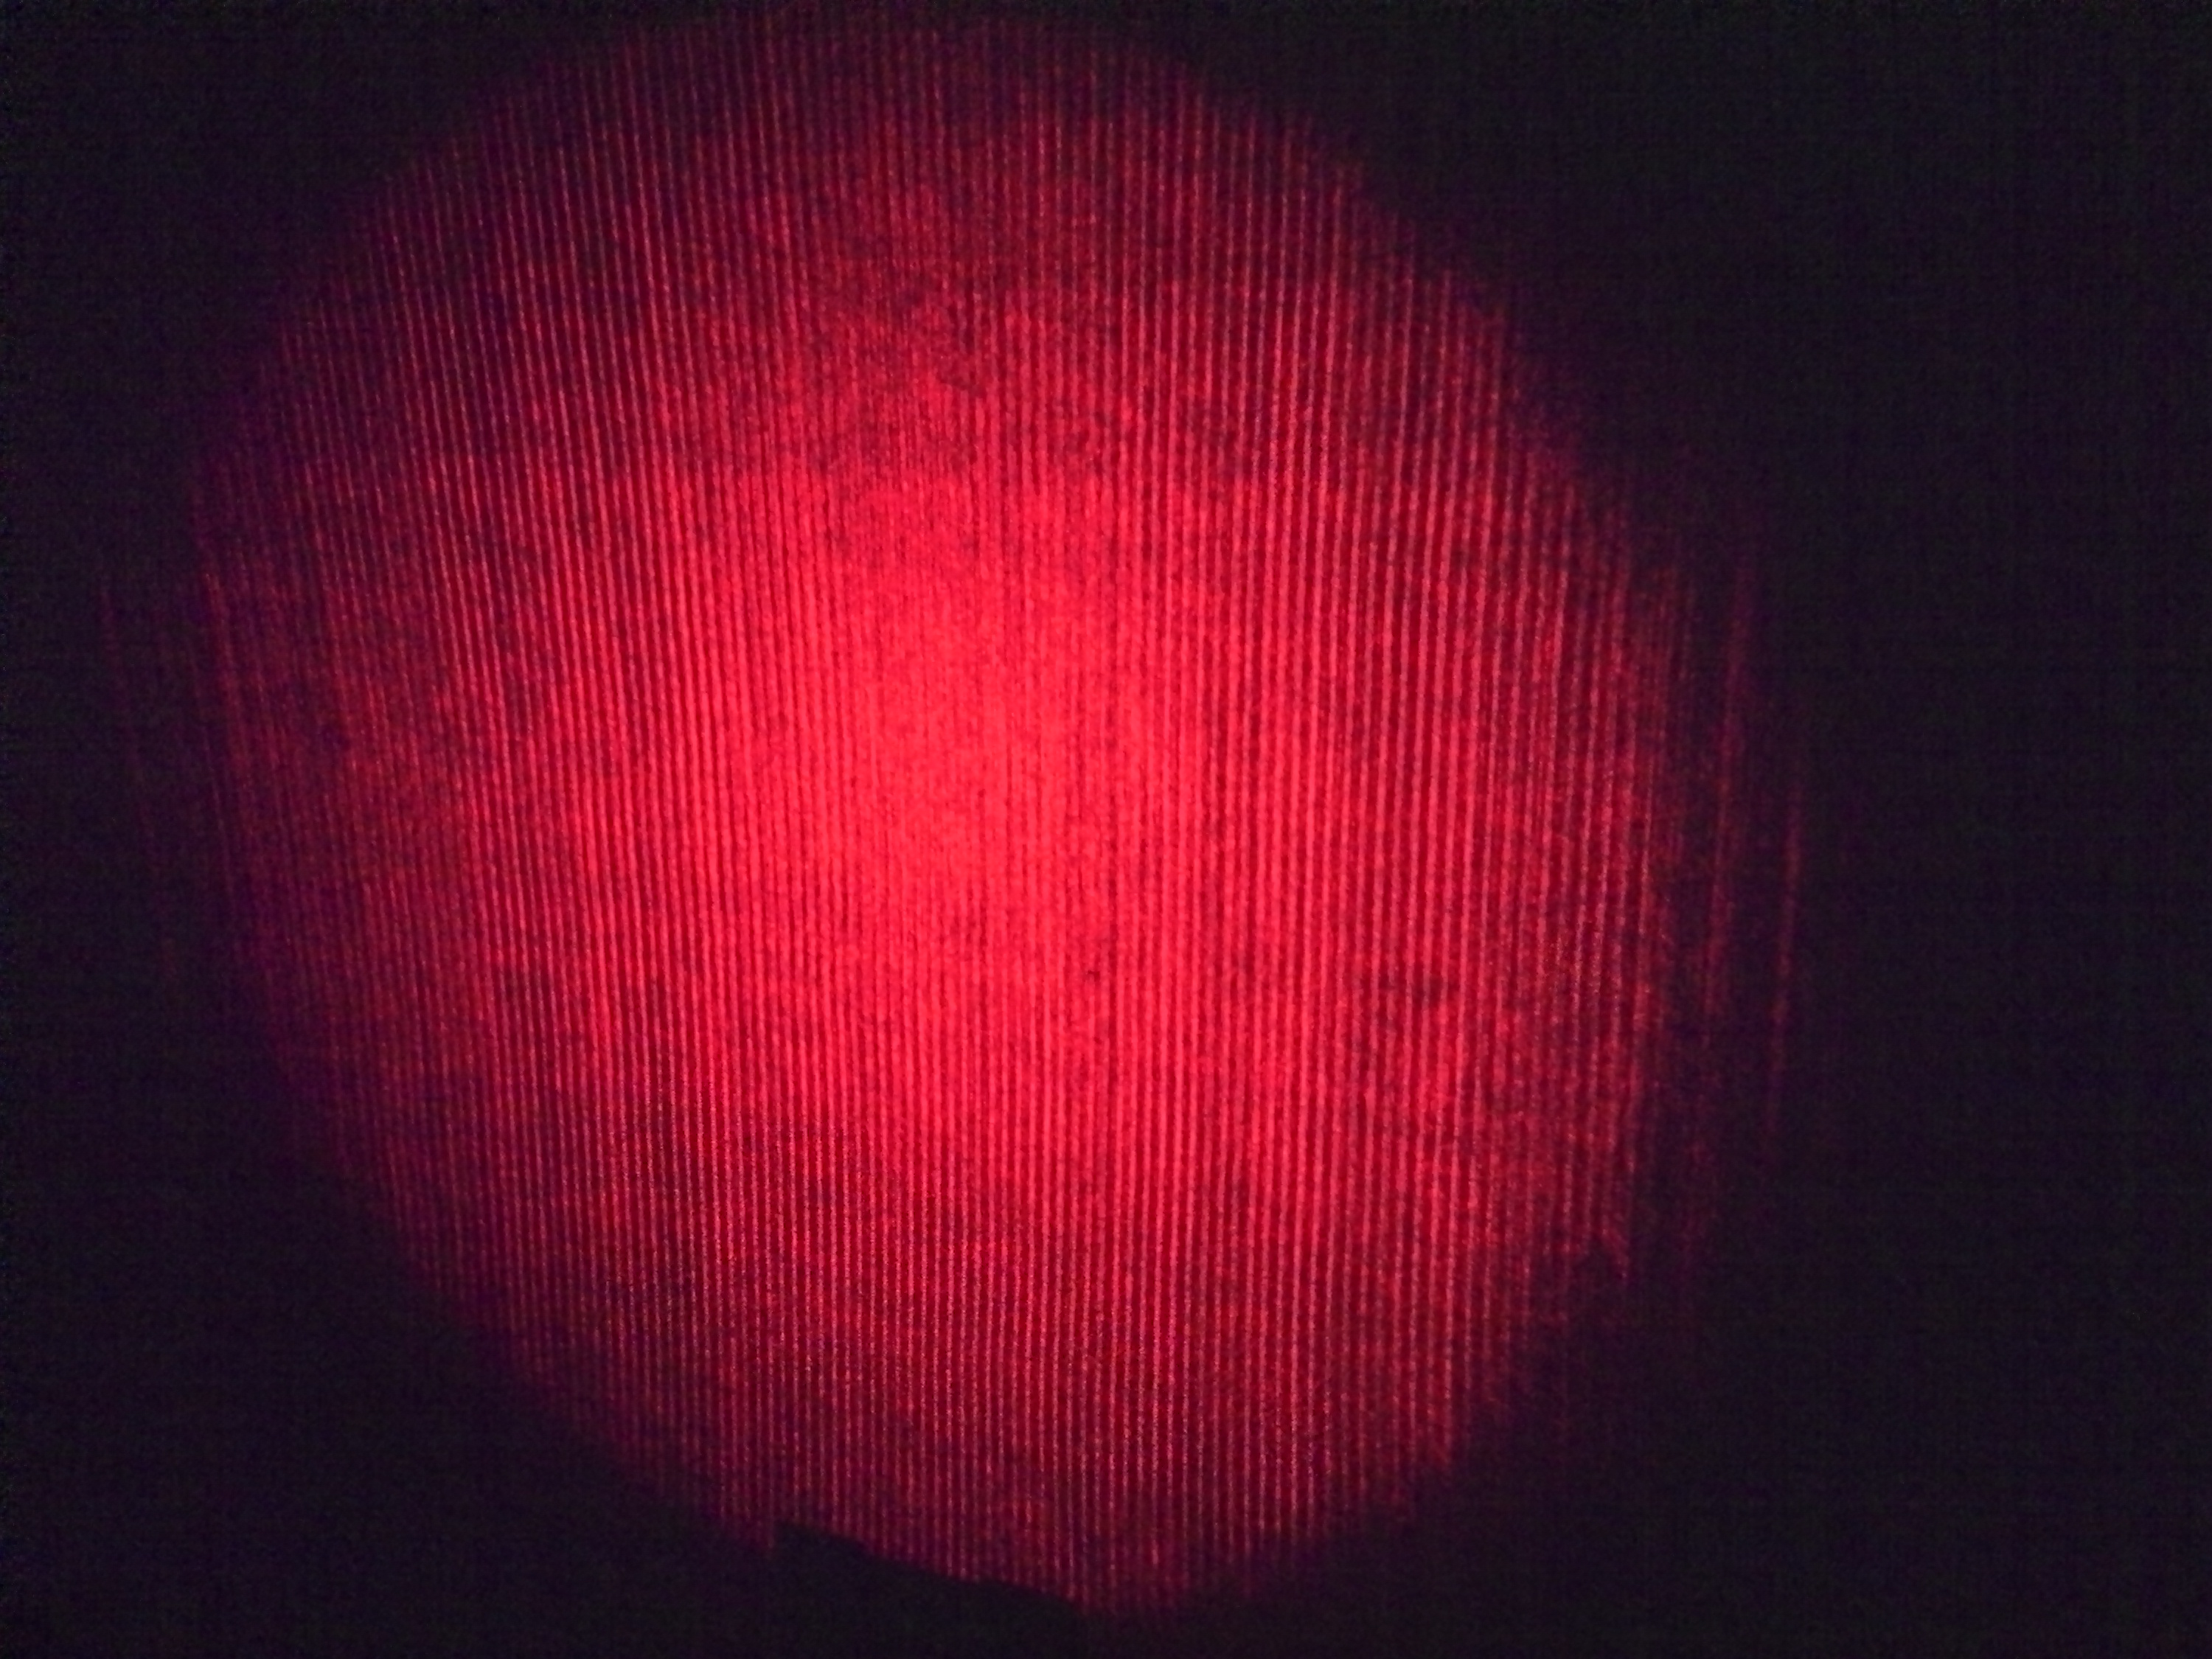
\includegraphics[width=\textwidth]{data/optics/04_Gitter_1D}
		\caption{Bild}
	\end{subfigure}
	\begin{subfigure}{0.49\textwidth}
		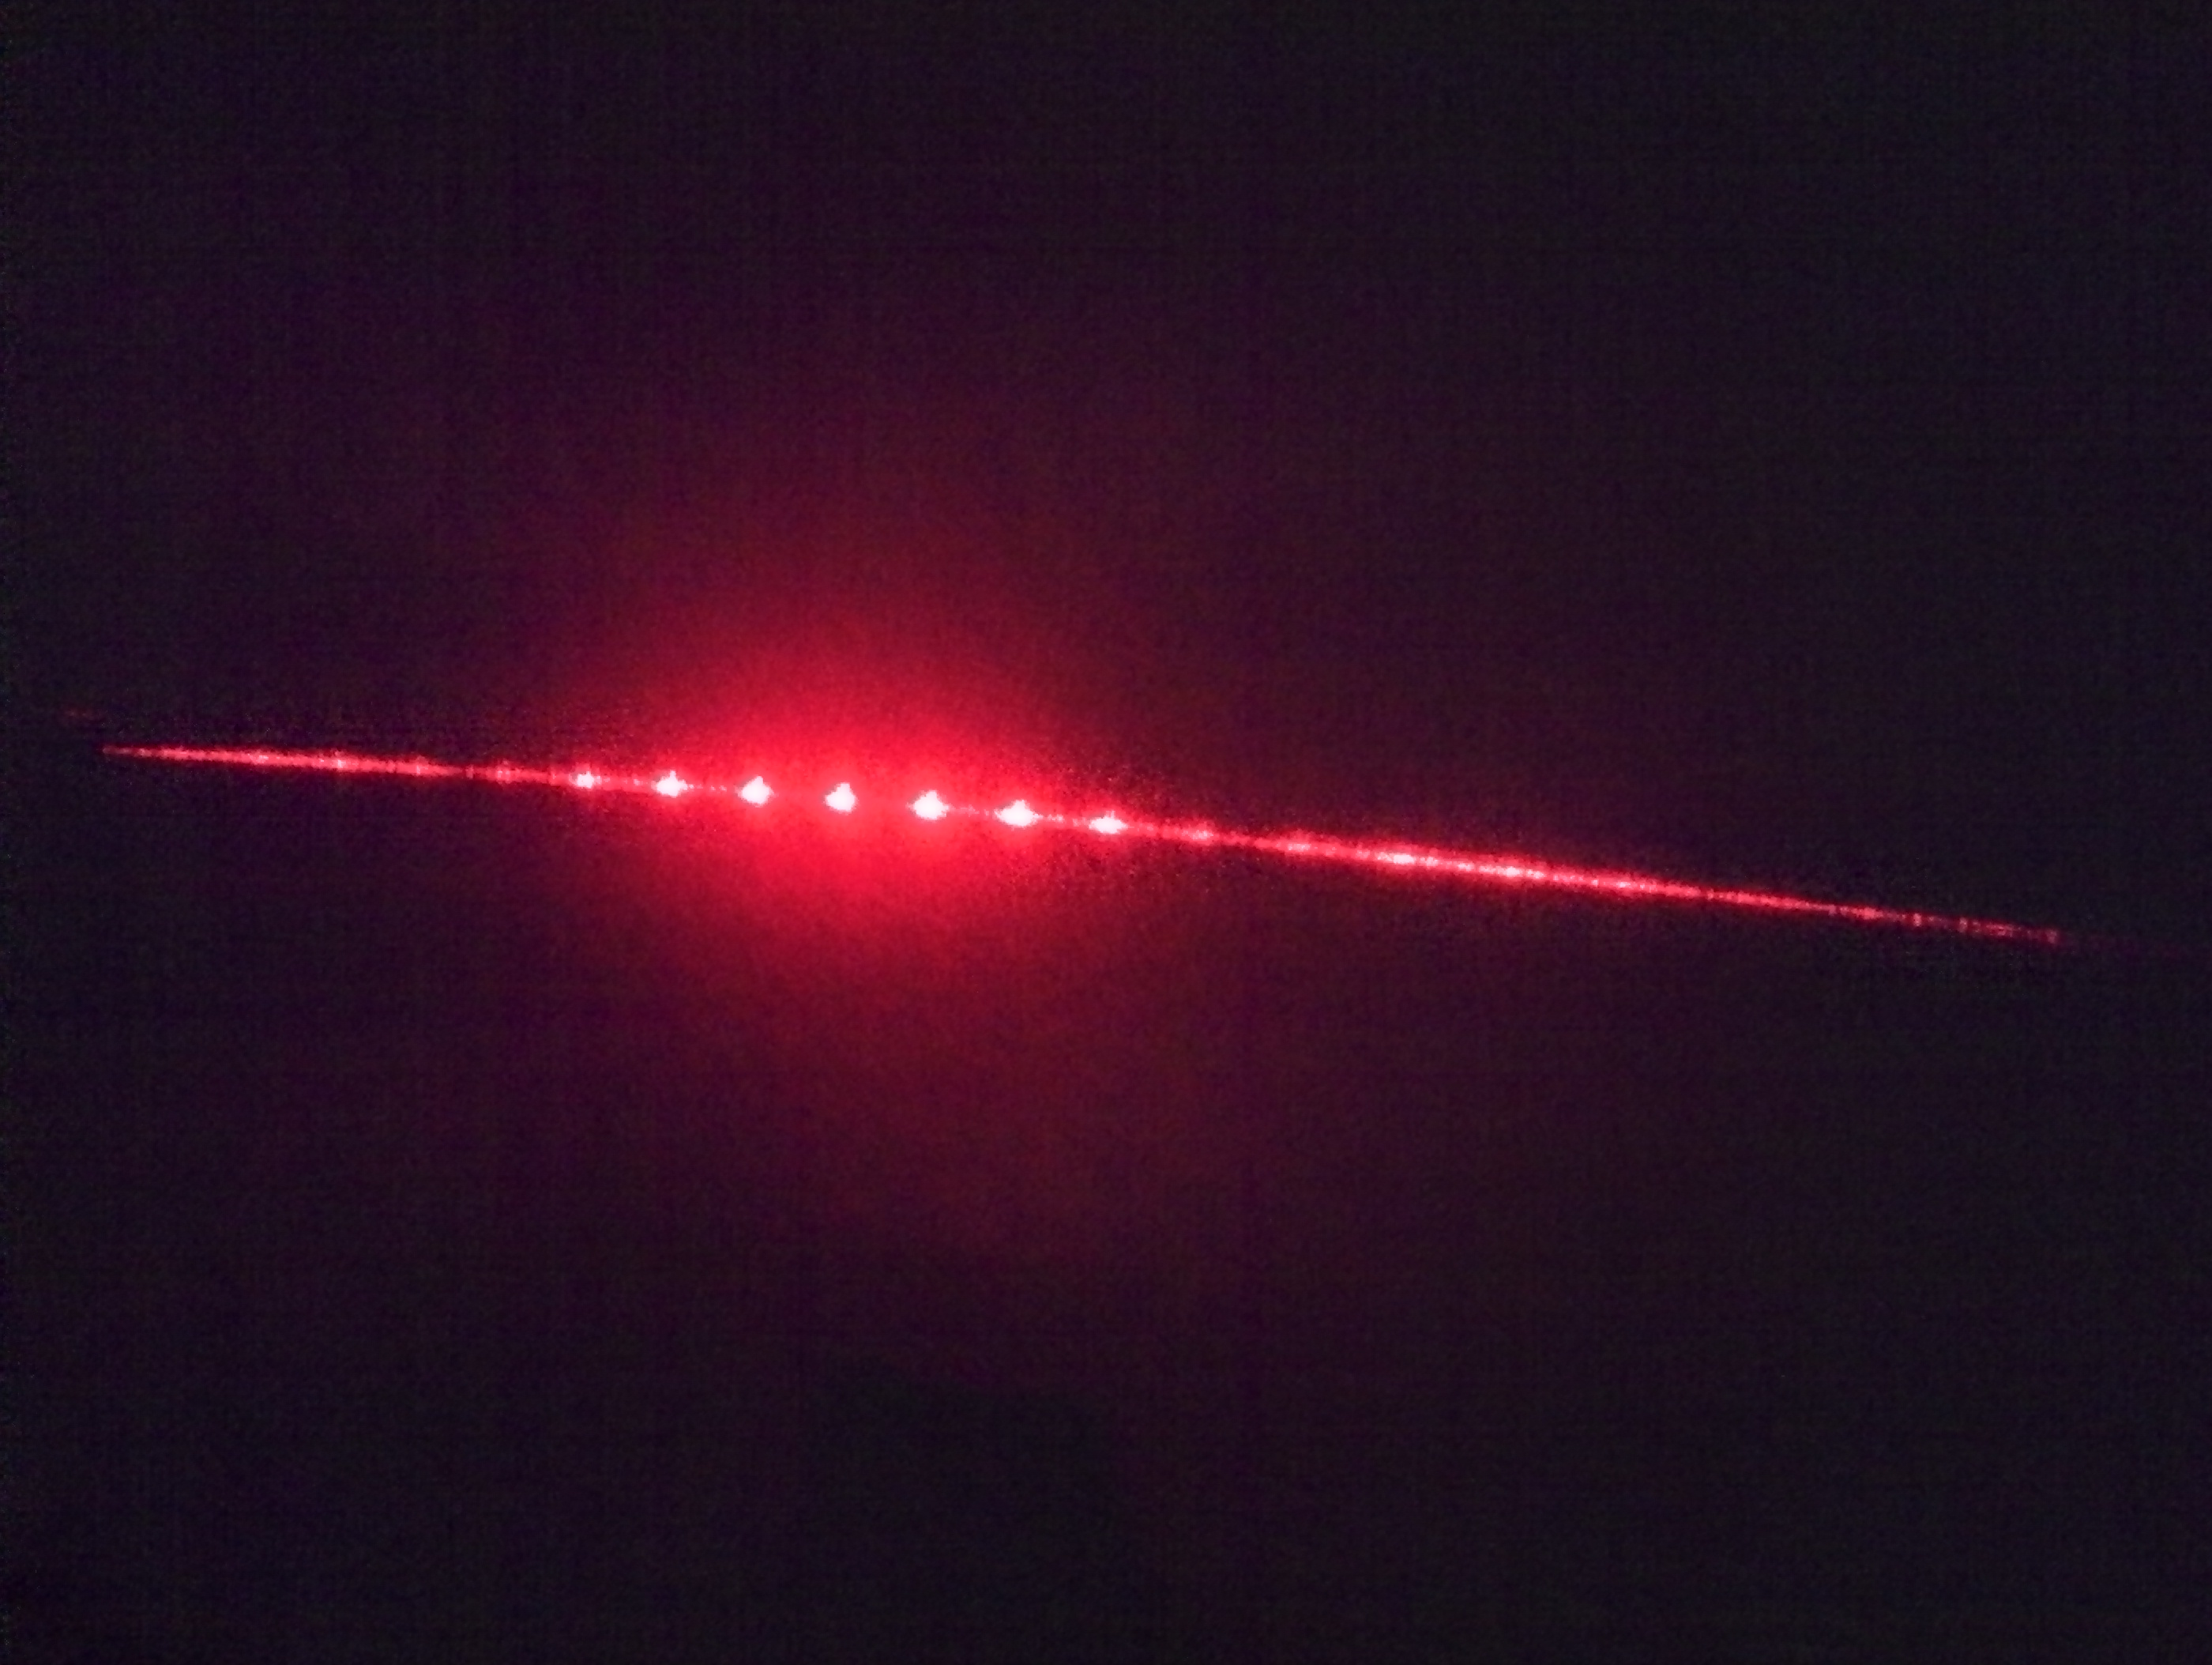
\includegraphics[width=\textwidth]{data/optics/04_Gitter_1D_Beugung}
		\caption{Beugungsbild} 		\label{fig:Gitter_BG}
	\end{subfigure}
	\caption{eindimensionales Gitter}		\label{fig:Gitter}
	\vspace{-1em}
\end{figure}

\begin{figure}[p]
	\centering
	\begin{subfigure}{0.49\textwidth}
		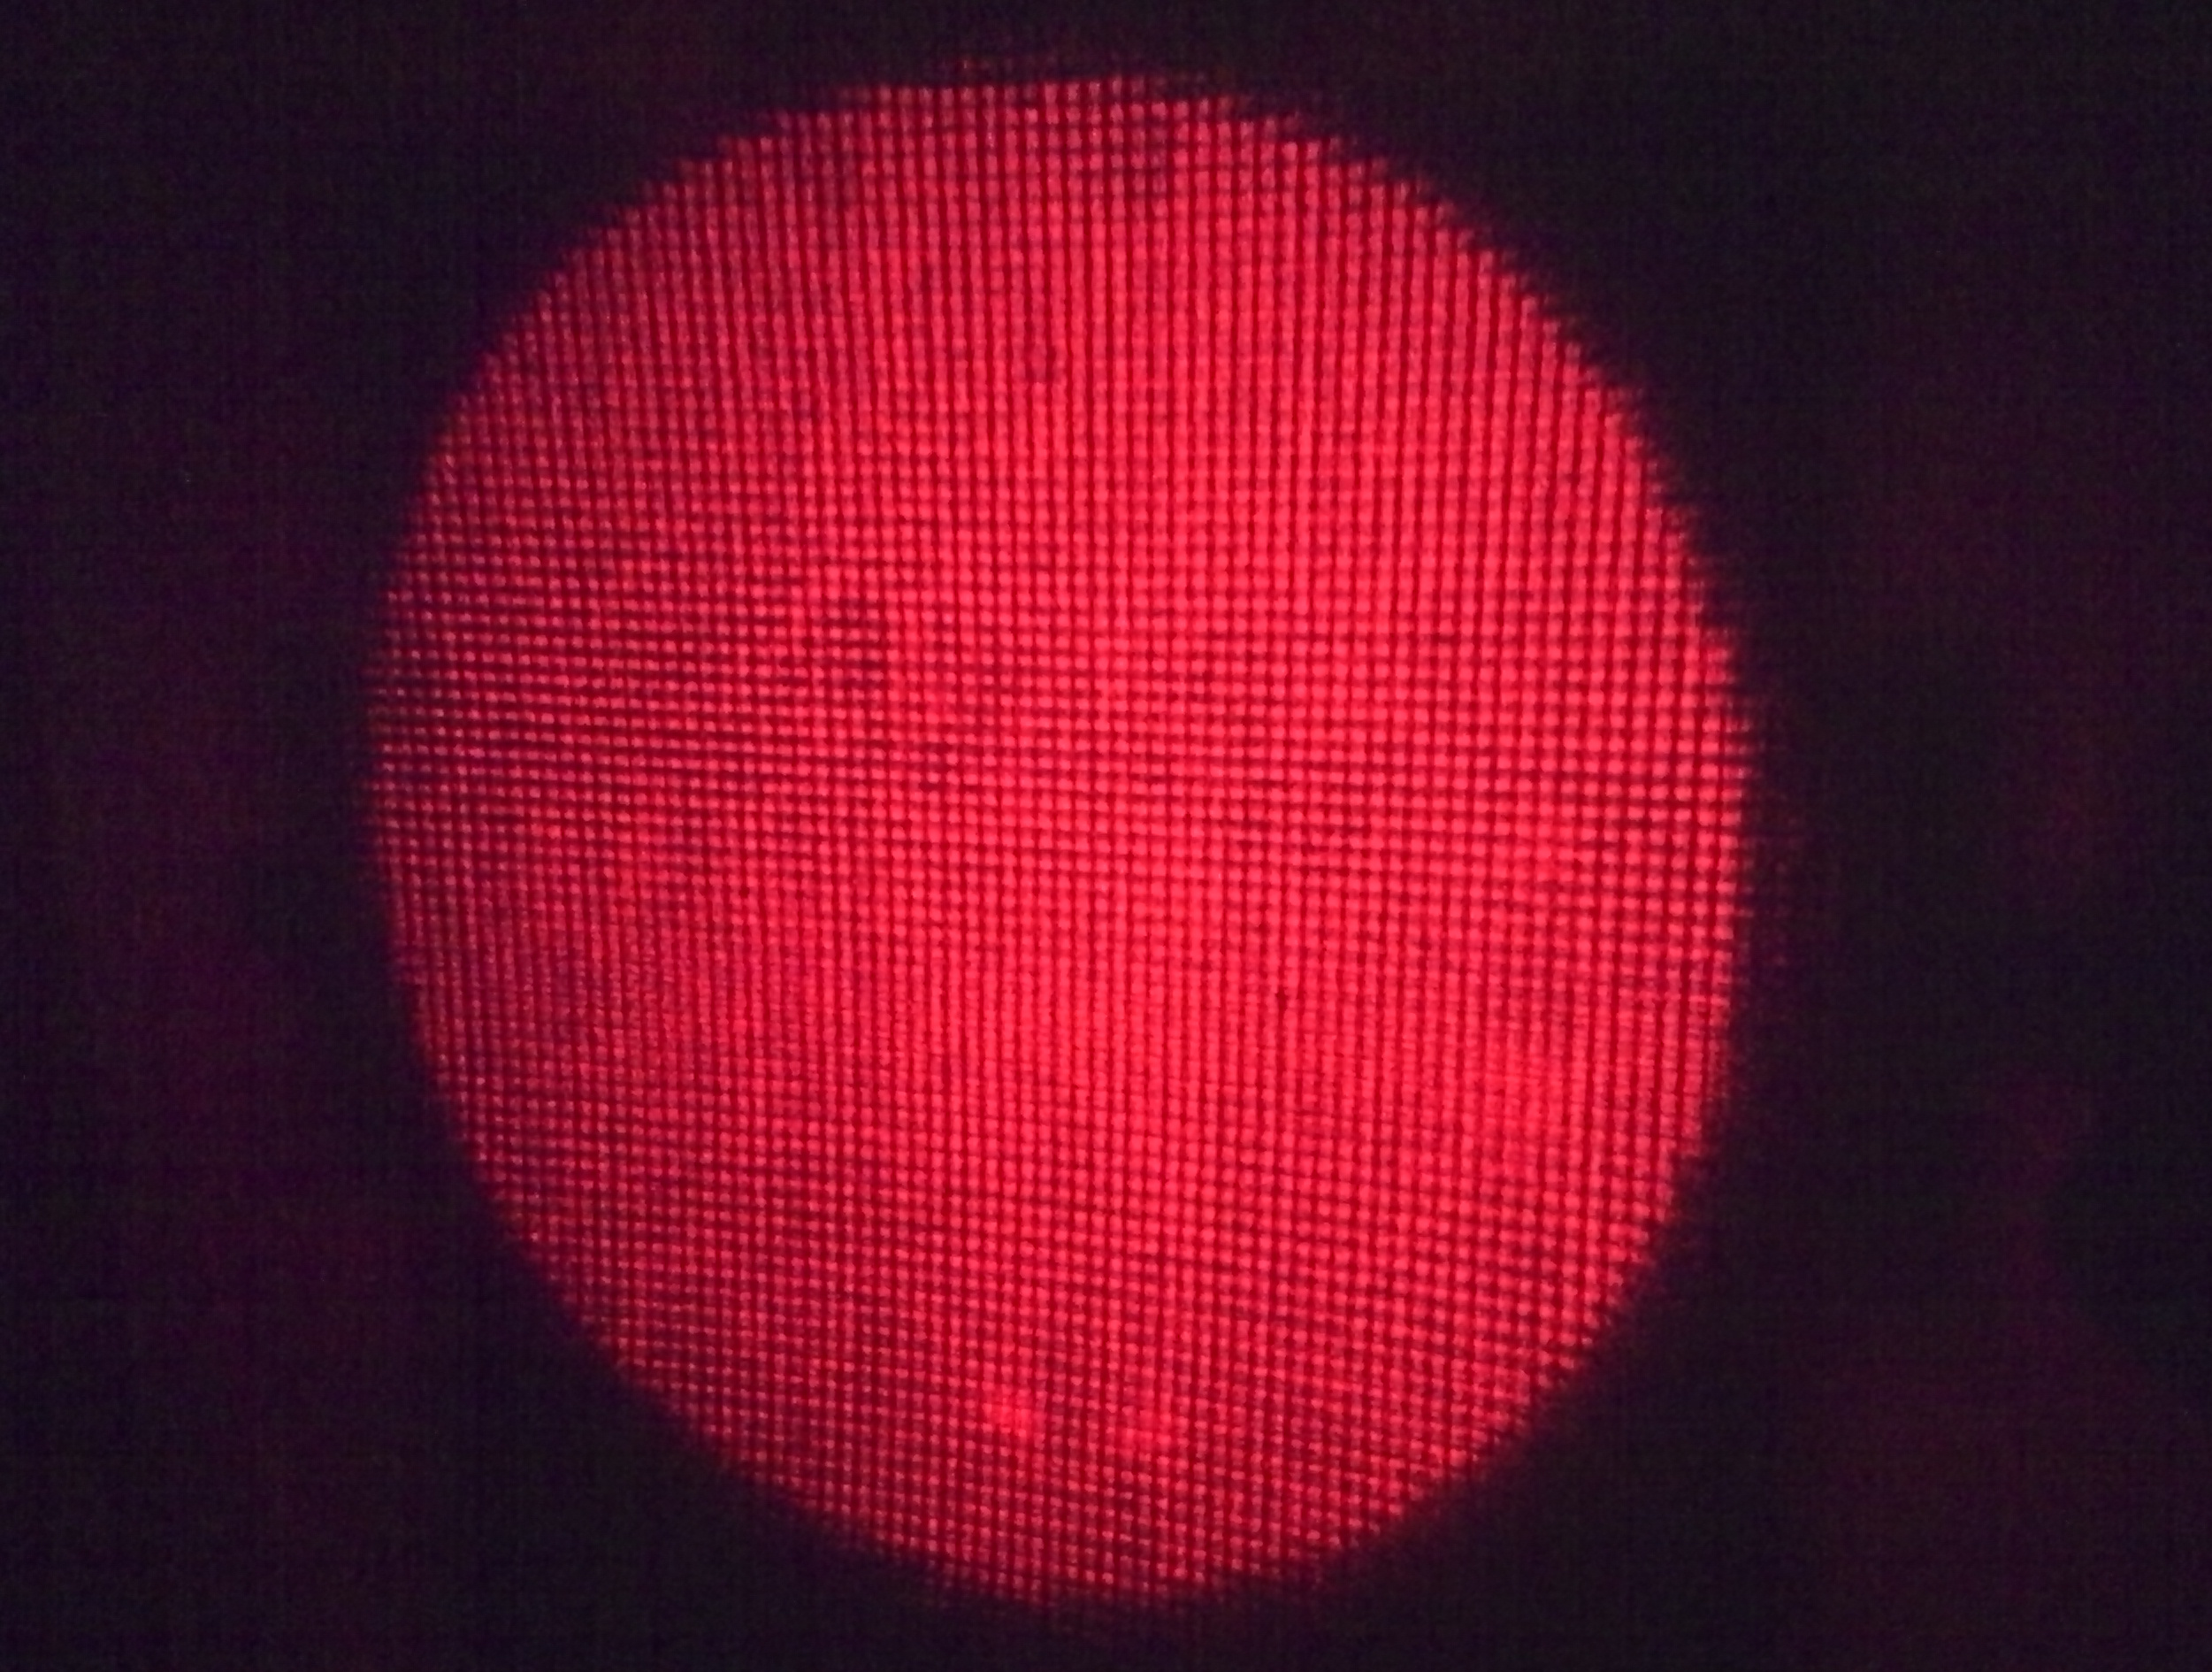
\includegraphics[width=\textwidth]{data/optics/05_Gitter_2D}
		\caption{Bild}
	\end{subfigure}
	\begin{subfigure}{0.49\textwidth}
		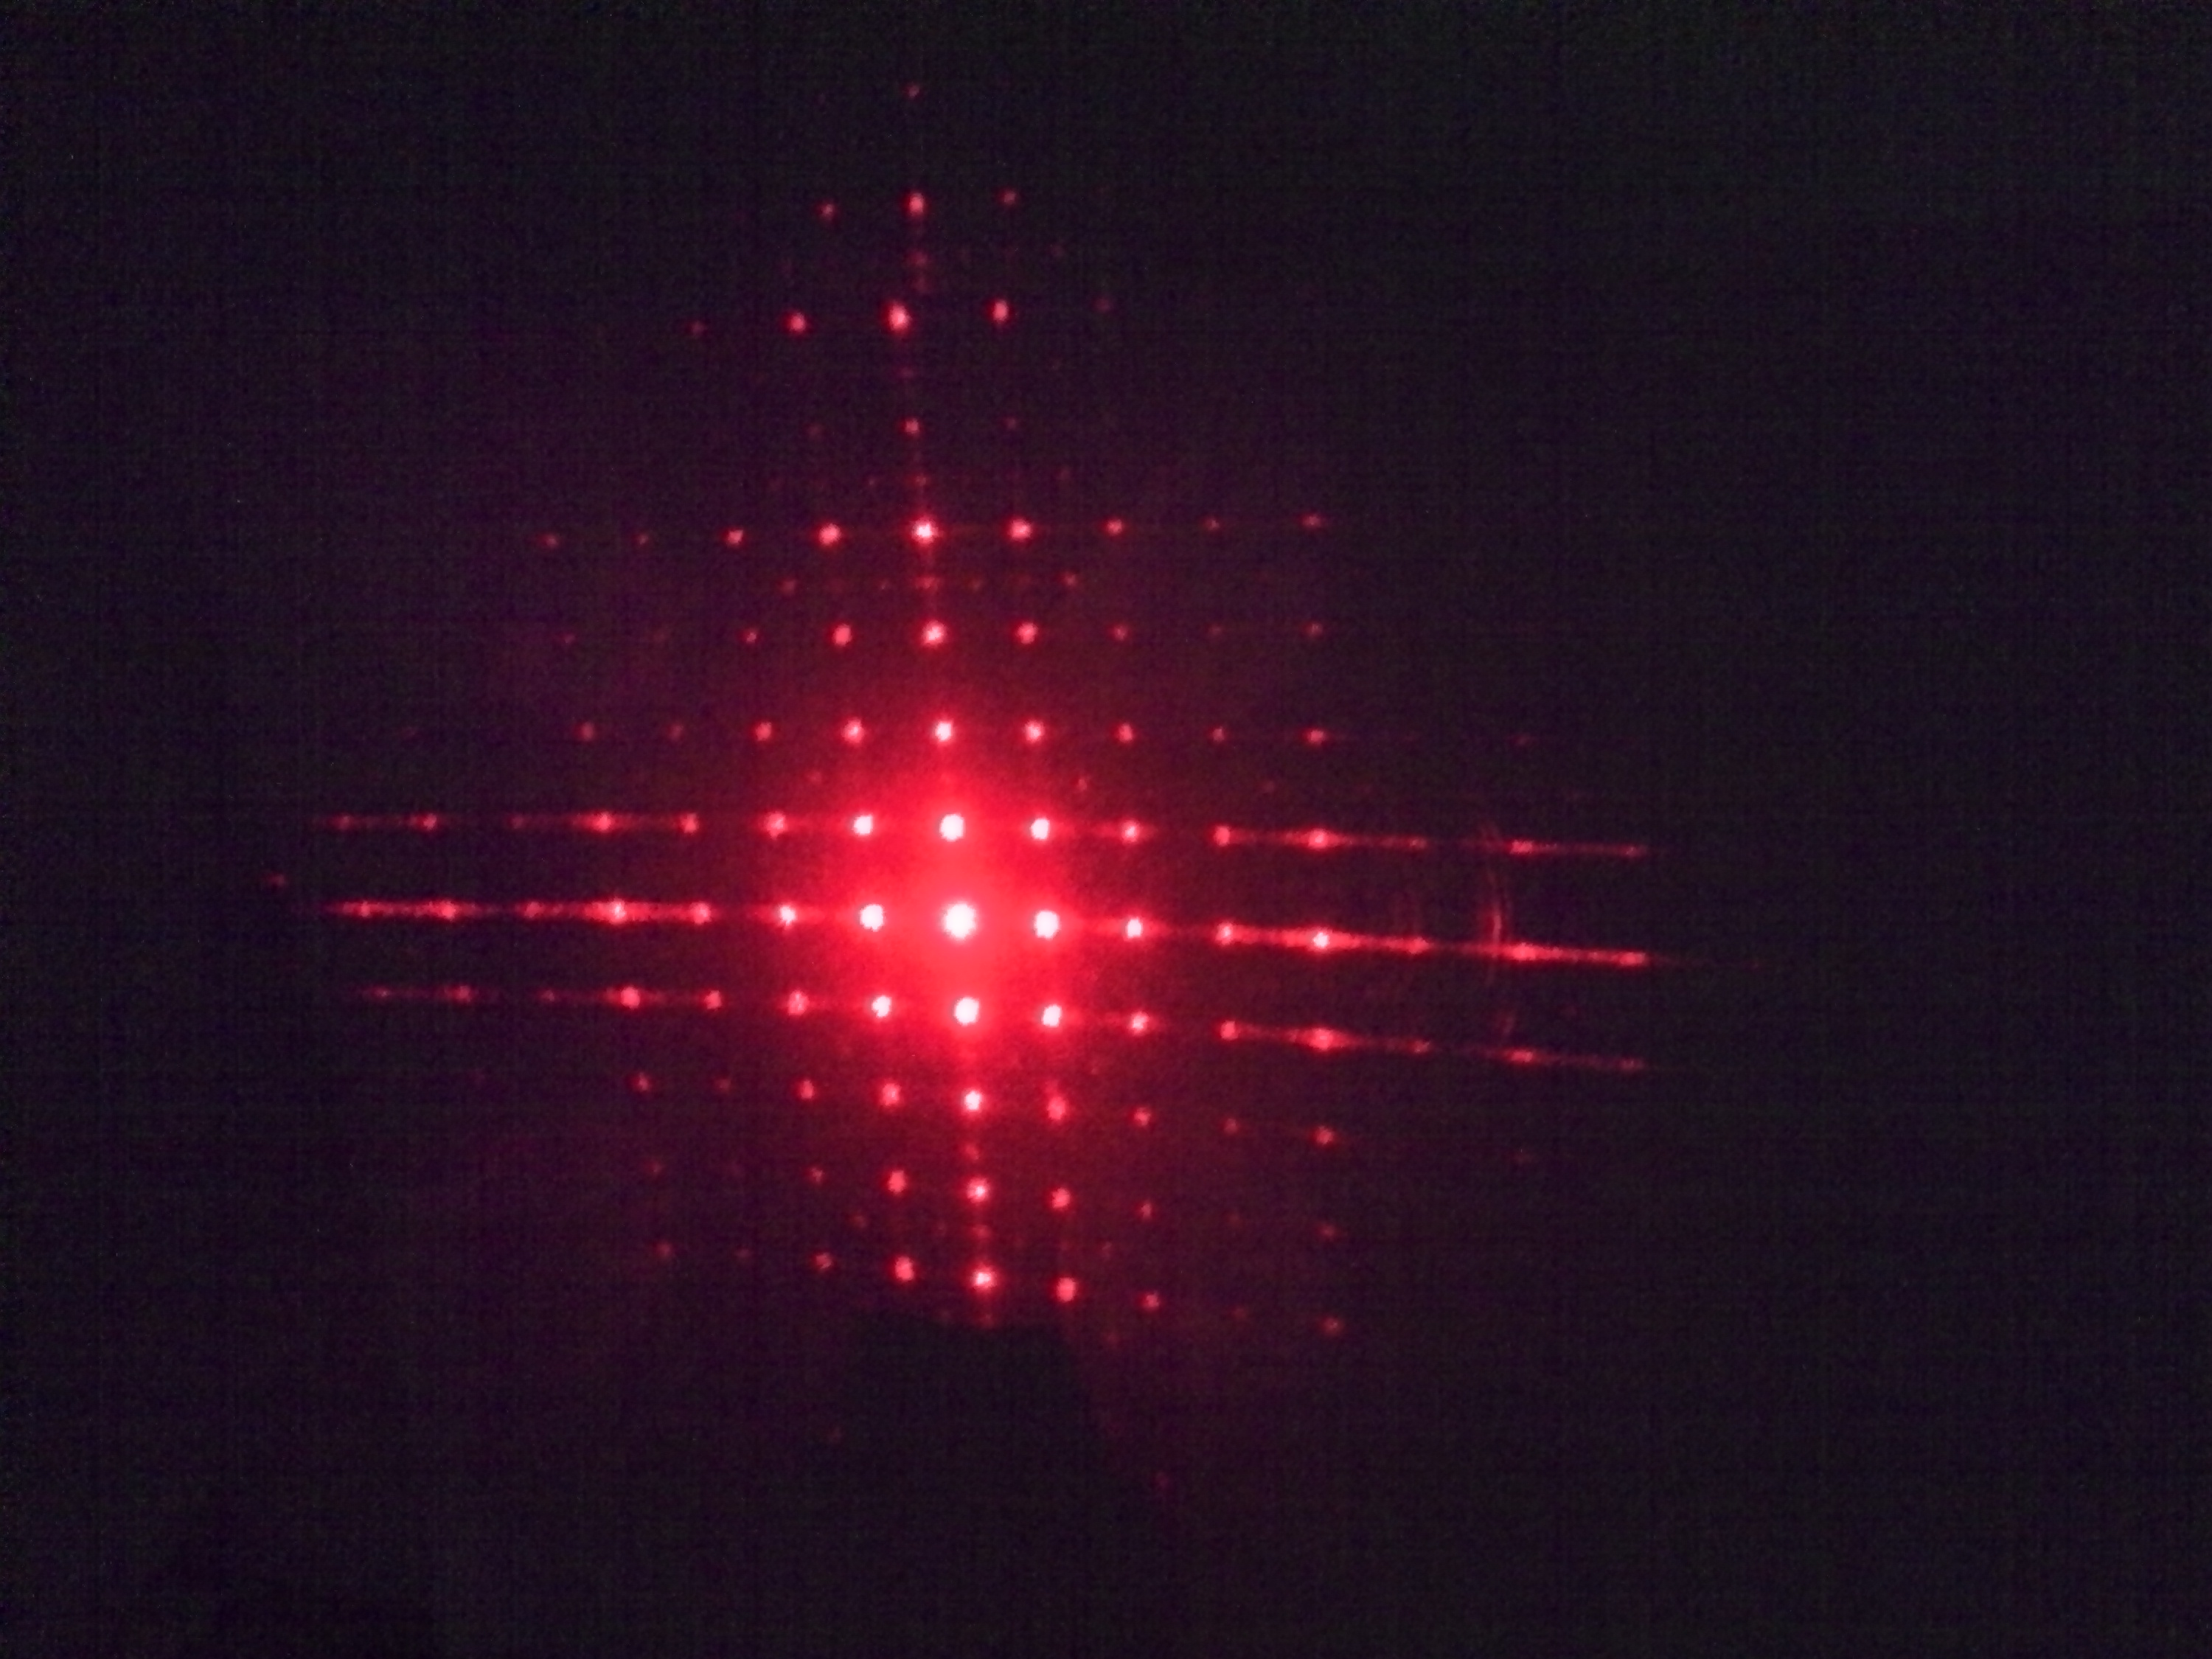
\includegraphics[width=\textwidth]{data/optics/05_Gitter_2D_Beugung}
		\caption{Beugungsbild}		 \label{fig:Gitter_2D_BG}
	\end{subfigure}
	\caption{zweidimensionales Gitter}	\label{fig:Gitter_2D}
	\vspace{-5em}
\end{figure}

Für den Einzelspalt erwarten wir als Intensitätsverlauf im Beugungsbild gemäß Gleichung \eqref{eq:sinc} den Sinus Cardinalis. Das charakteristische Merkmal, das breite Hauptmaximum, ist in unserem Photo jedoch nicht richtig erkennbar (siehe Abb. \ref{fig:Einzel_BG}). Wir vermuten, dass dies am Spalt selbst liegt -- als wir diesen gegen das Licht hielten, war eine schwache zweite Linie erkennbar. Bei einem Doppelspalt wäre das Hauptmaximum gleich breit wie die Nebenmaxima, was das beobachtete Muster erklären würde.

Das Beugungsbild eines perfekten Gitters wäre ein Delta-Kamm, durch die endliche Spaltbreite ist diesem eine $\sinc$-Funktion als Hüllkurve überlagert (Abb. \ref{fig:Gitter_BG}). Da wir den reziproken Raum abbilden, sind kleine Strukturen im Beugungsbild groß und umgekehrt -- da die Spaltbreite deutlich kleiner ist als der Spaltabstand, ist die Hüllkurve breit gegenüber dem Abstand der Maxima.

Das 2D-Gitter ist die Überlagerung zweier 1D-Gitter, somit ist das Beugungsbild ein Punktgitter entlang zweier Achsen (Abb. \ref{fig:Gitter_2D_BG}). Aus diesem ist anhand der gleichen Abstände erkennbar, dass die zwei Gitterkonstanten gleich sind (Netz mit quadratischen Maschen).


\newpage
\subsubsection{Einstein-Portrait}
Auf einem Dia ist das Portrait Einsteins abgebildet, allerdings ist dieses durch ein Gitter überlagert, wodurch man nur ein verschwommenes Bild erhält (Abb. \ref{fig:Einstein_B}). Da das Gitter deutlich feiner ist als das Portrait, zeigen sich im Beugungsbild die typischen Punktreflexe eines Gitters (Abb. \ref{fig:Einstein_BG}). Gemäß dem Faltungstheorem enthält jeder dieser Reflexe die Information des Portraits.

Selektieren wir durch eine Rechteckblende im Brennpunkt von $L_3$ ausschließlich das Hauptmaximum (Abb. \ref{fig:Einstein_hell_B}), so entfällt die Information des Gitters und erhalten ein gefiltertes Bild. Diese Methode wird als Hellfeld-Mikroskopie bezeichnet.

Verschieben wir die Rechteckblende so, dass lediglich das Licht eines Nebenmaximums hindurch gelangt (Abb. \ref{fig:Einstein_dunkel_B}), so sehen wir im Bild nur das am Objekt gestreute Licht und sehen folglich das Portrait auf dunklem Hintergrund, daher auch der Name Dunkelfeld-Mikroskopie. Der Kontrast ist typischerweise besser, allerdings ist die Intensität des gestreuten Lichts verständlicherweise deutlich geringer als im Hellfeld.

\begin{figure}[p]
	\centering
	\begin{subfigure}[b]{0.49\textwidth}
		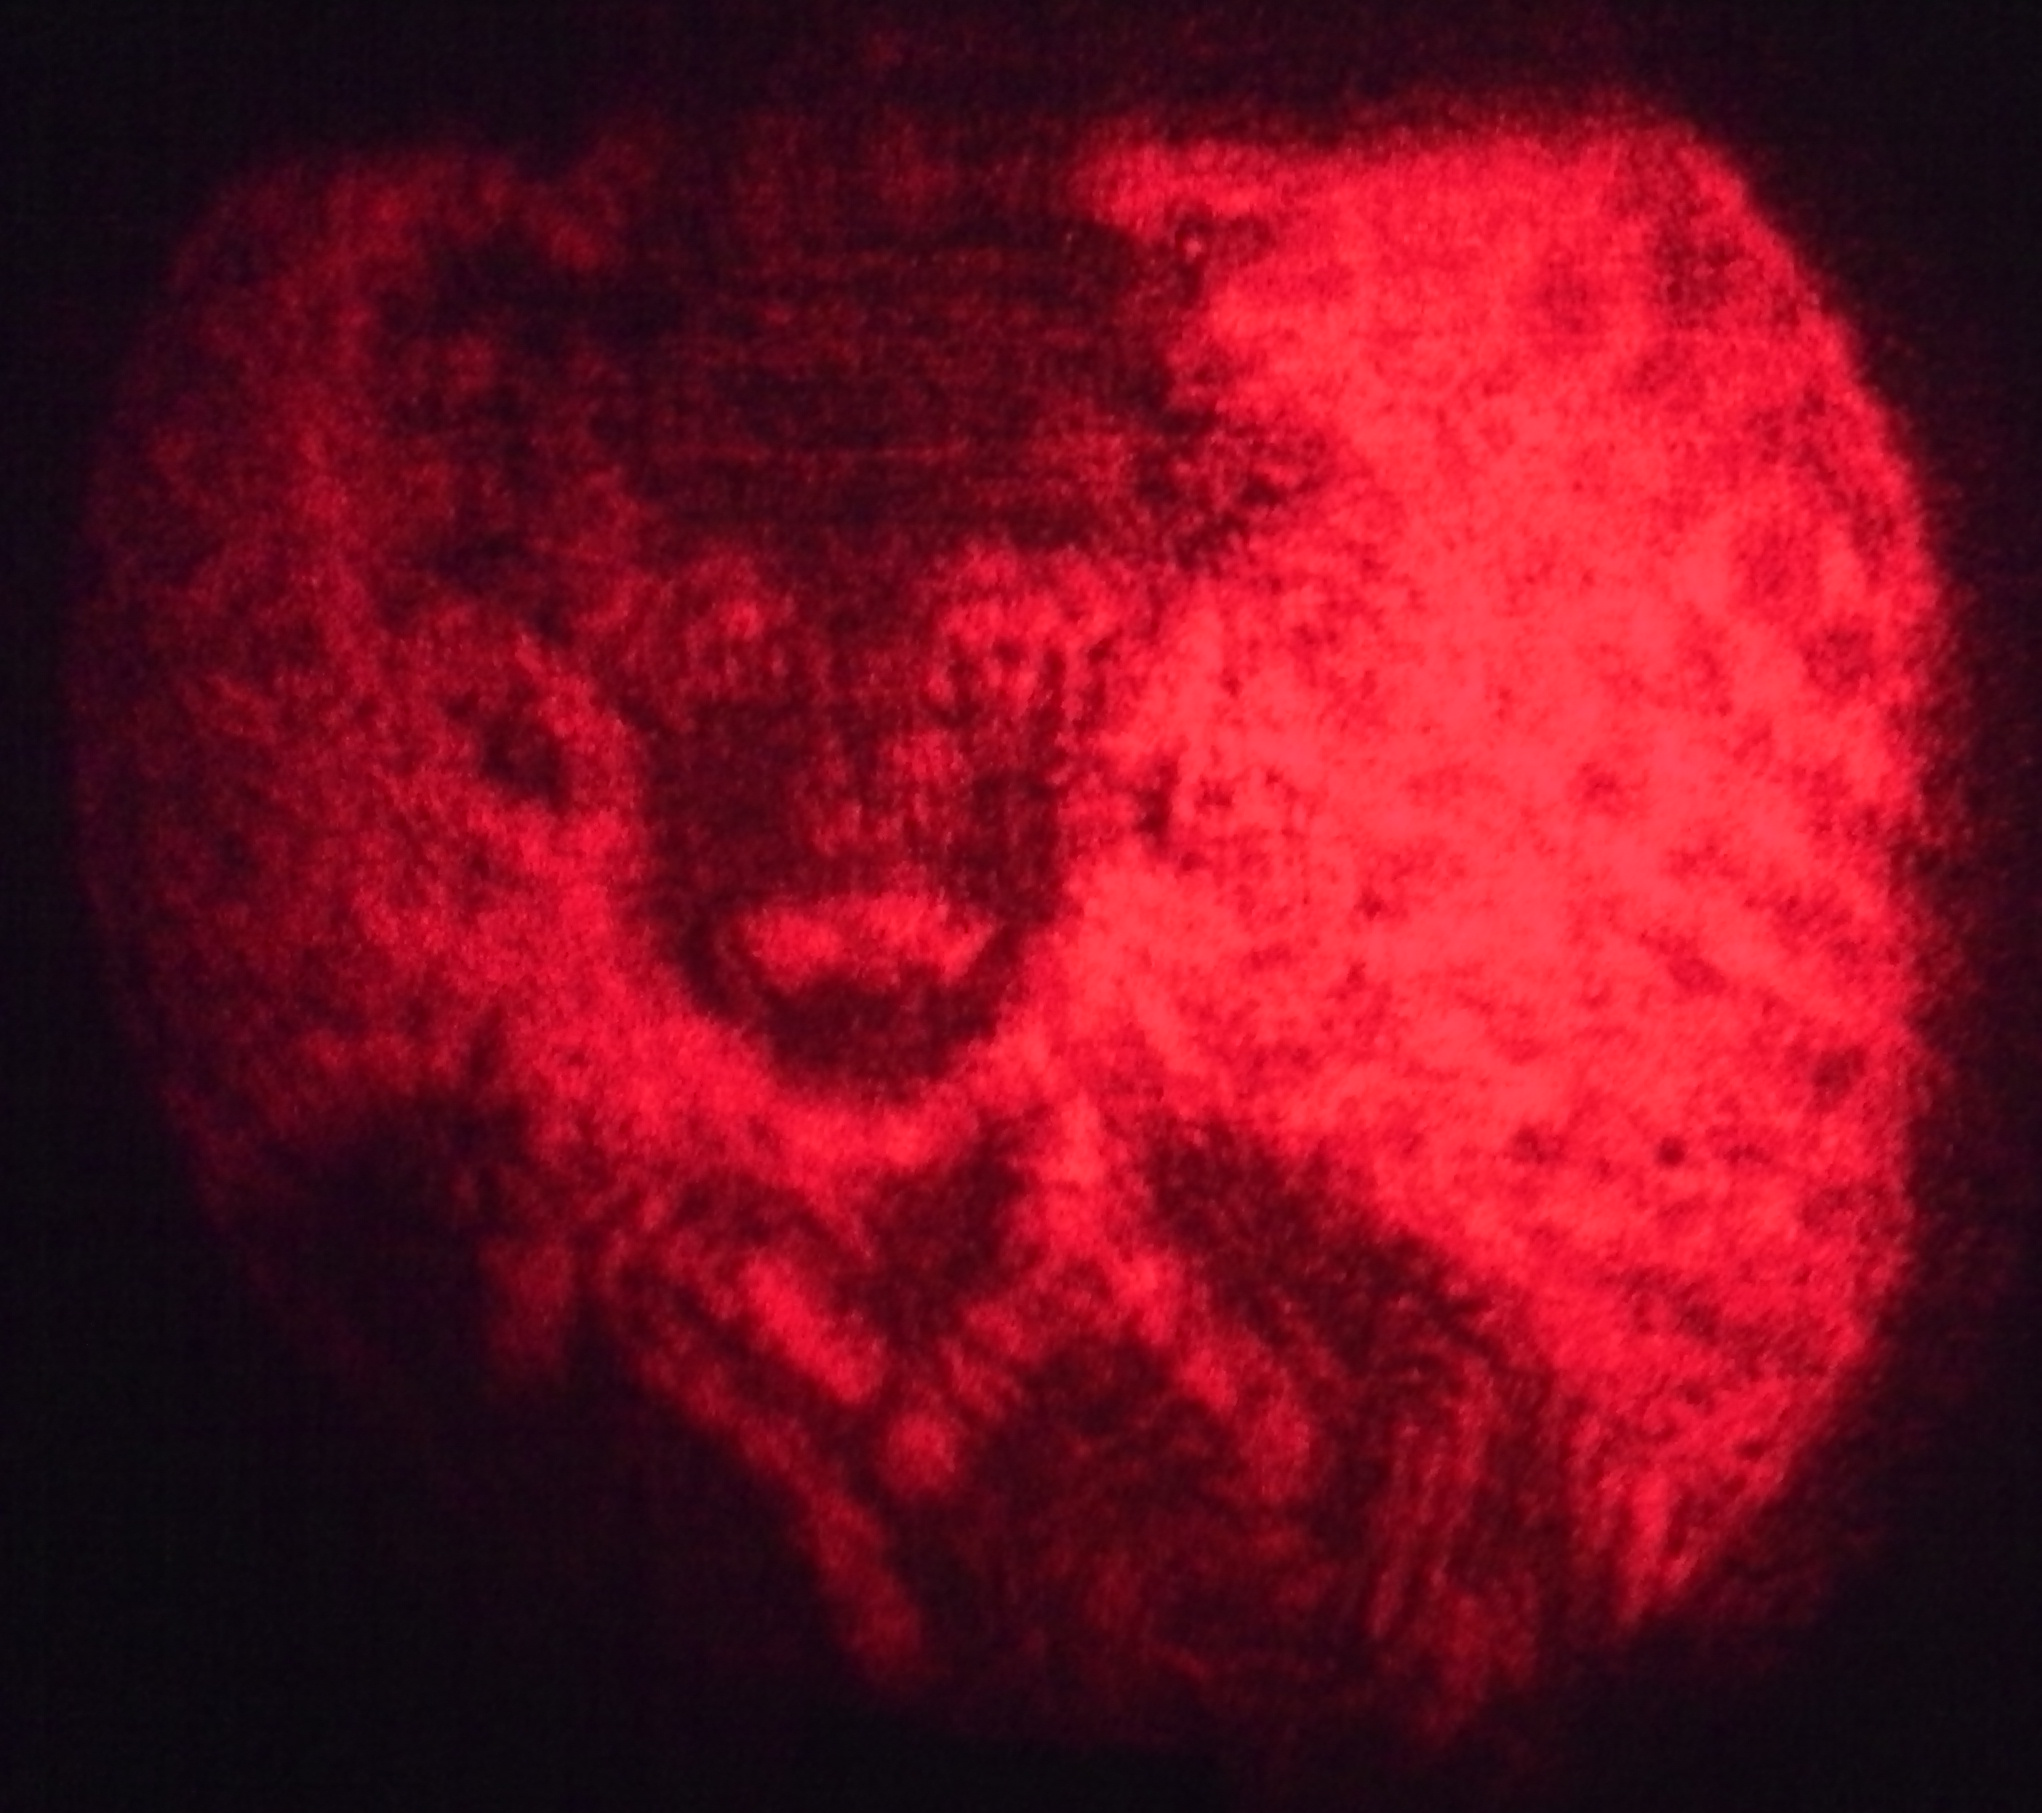
\includegraphics[width=\textwidth]{data/optics/06_Einstein_Bild}
		\caption{Bild}				\label{fig:Einstein_B}
	\end{subfigure}
	\begin{subfigure}[b]{0.49\textwidth}
		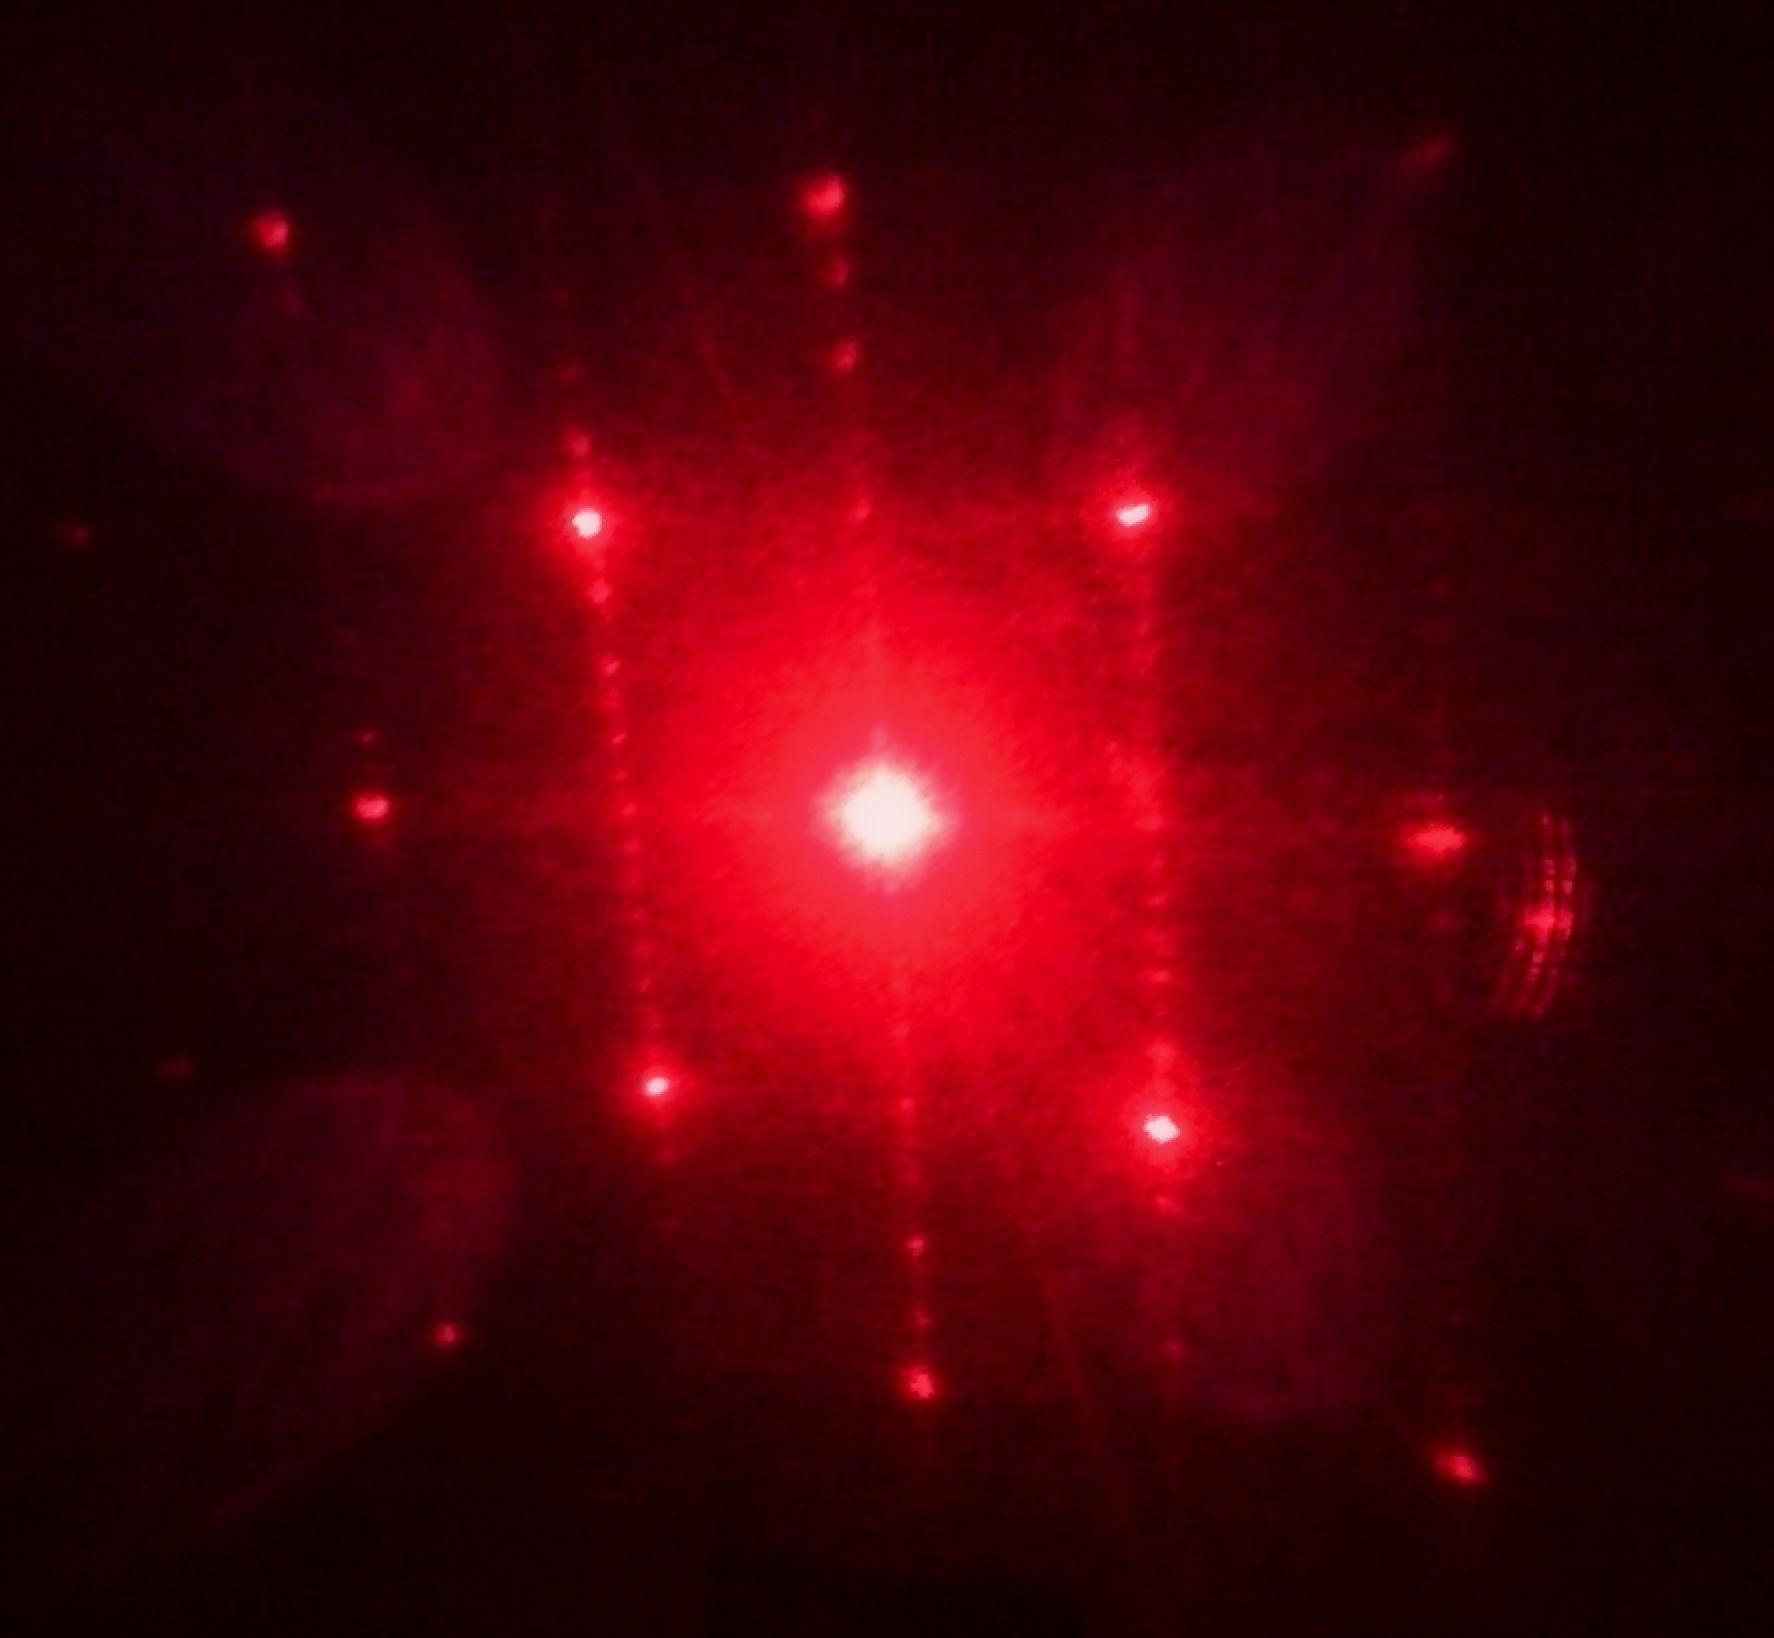
\includegraphics[width=\textwidth]{data/optics/06_Einstein_Beugung}
		\caption{Beugungsbild} 		\label{fig:Einstein_BG}
	\end{subfigure}
	\caption{Einstein-Portrait}			\label{fig:Einstein}
	\vspace{-1em}
\end{figure}

\begin{figure}[p]
	\centering
	\begin{subfigure}{0.49\textwidth}
		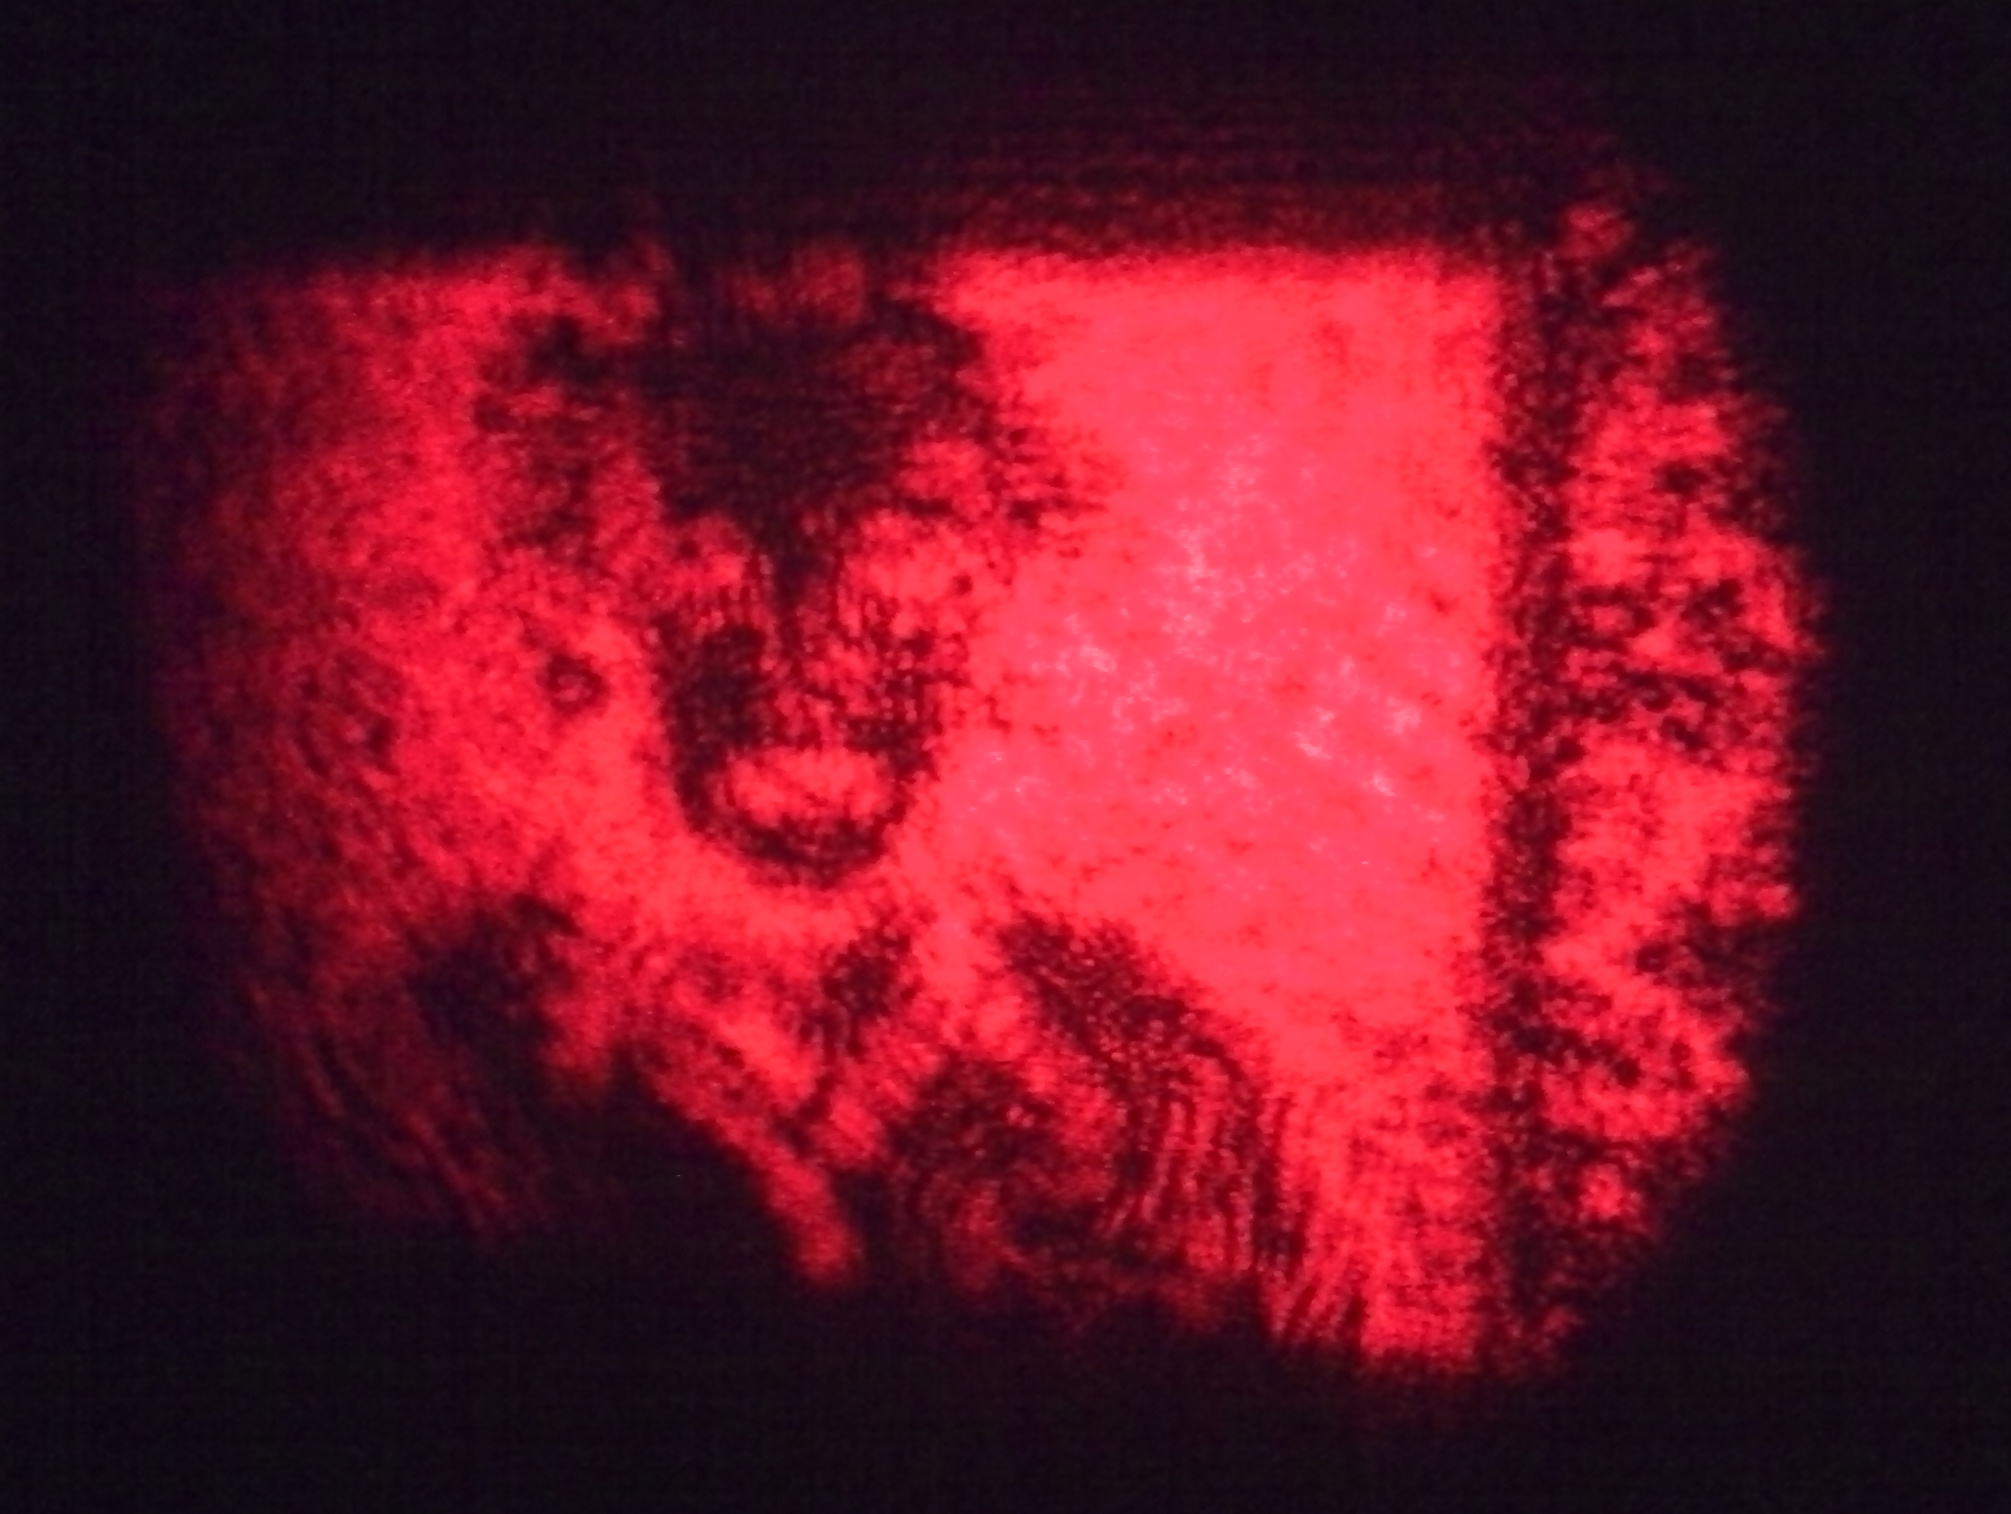
\includegraphics[width=\textwidth]{data/optics/06_Einstein_Hell_Bild}
		\caption{Hellfeld-Bild}				\label{fig:Einstein_hell_B}
	\end{subfigure}
	\begin{subfigure}{0.49\textwidth}
		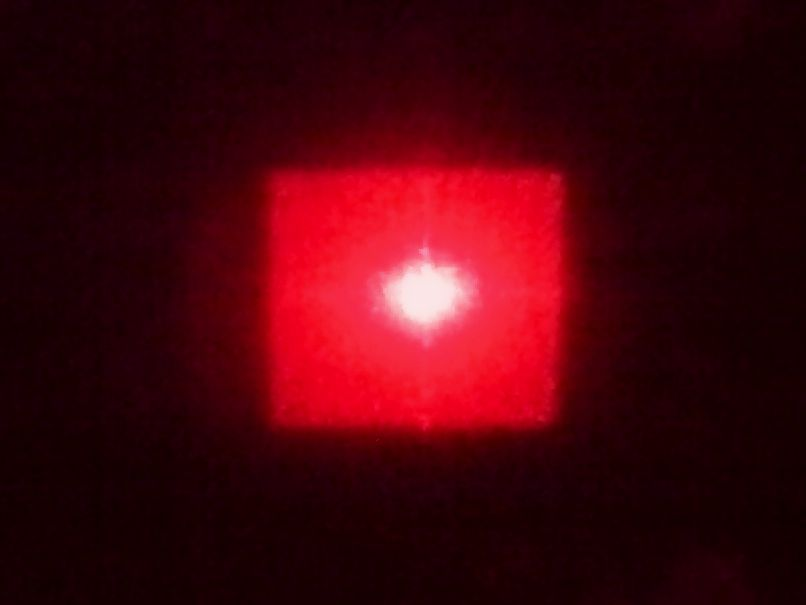
\includegraphics[width=\textwidth]{data/optics/06_Einstein_Hell_Beugung}
		\caption{Beugungsbild: Hauptmaximum}	\label{fig:Einstein_hell_BG}
	\end{subfigure}
	\caption{Einstein-Portrait im Hellfeld}		\label{fig:Einstein_hell}
	\vspace{-1em}
\end{figure}

\begin{figure}[p]
	\centering
	\begin{subfigure}{0.49\textwidth}
		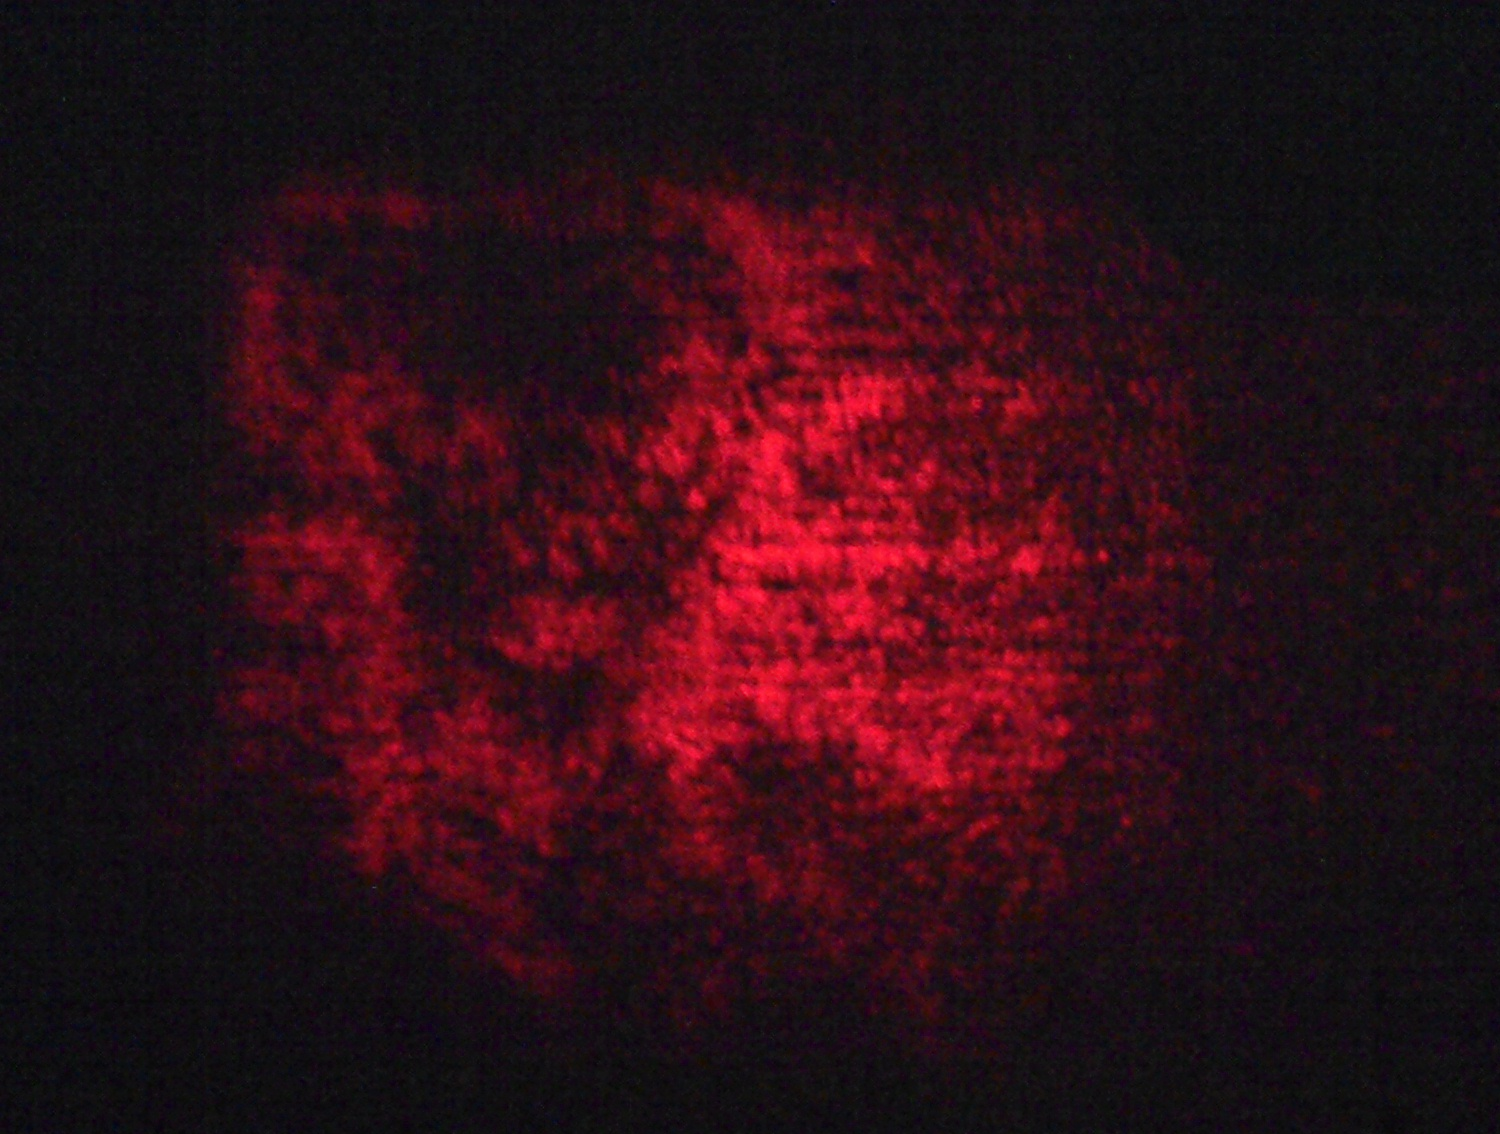
\includegraphics[width=\textwidth]{data/optics/06_Einstein_Dunkel_Bild}
		\caption{Dunkelfeld-Bild}				 \label{fig:Einstein_dunkel_B}
	\end{subfigure}
	\begin{subfigure}{0.49\textwidth}
		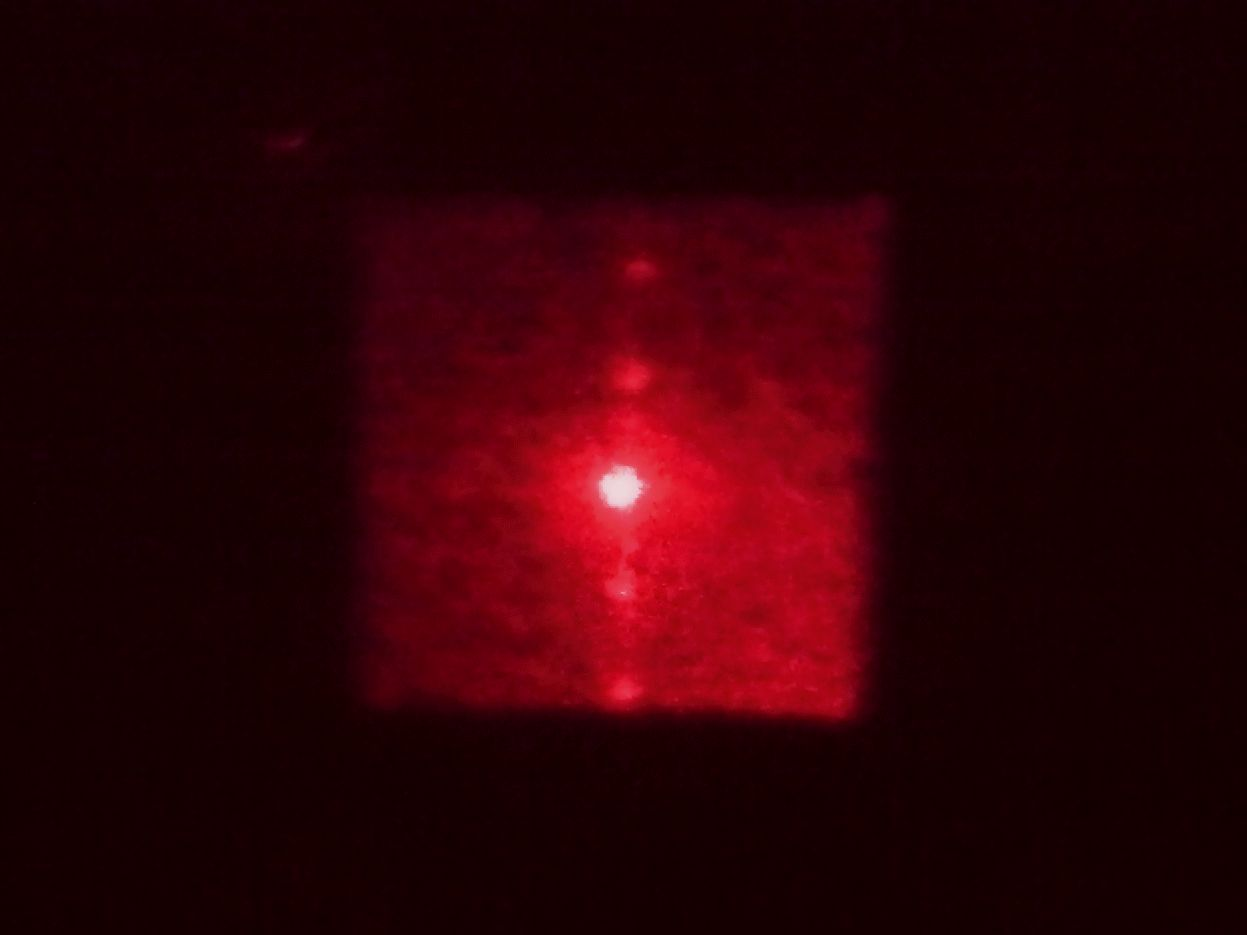
\includegraphics[width=\textwidth]{data/optics/06_Einstein_Dunkel_Beugung}
		\caption{Beugungsbild: Nebenmaximum}	 \label{fig:Einstein_dunkel_BG}
	\end{subfigure}
	\caption{Einstein-Portrait im Dunkelfeld}		\label{fig:Einstein_dunkel}
	\vspace{-5em}
\end{figure}




\newpage
\subsection{Transmissions-Elektronenmikroskop}
Das TEM ist analog zum Lichtmikroskop aufgebaut, wobei wir Elektronen anstelle von Photonen verwenden, da ihre De-Broglie-Wellenlänge
\begin{equation}
\lambda = \frac{h}{p} \stackrel{200\,\kilo\electronvolt}{=} 2,5\,\pico\metre
\end{equation}
ein deutlich höheres Auflösungsvermögen ermöglicht.

Der Versuchsaufbau ist in Abbildung \ref{fig:setup} dargestellt, die Linsen sind dabei als Magnetlinsen ausgeführt. Da letztere nur als Sammellinse (und nicht als Zerstreuungslinse) dienen können, sind die gewöhnlichen Korrekturen (z.B. Dubletts gegen chromatische Aberration) nicht anwendbar. Anstelle dessen wird das Energiespektrum der Elektronen eingeschränkt (Dispersion weniger relevant) und achsferne Strahlen durch zwei Multipole (Stigmatoren) korrigiert.

 Ziel ist es, ein metallisches Pulver zu identifizieren, dabei kommen die festen Edelmetalle in Frage: \textsf{Ru, Os} (hpc) und \textsf{Rh, Pd, Ag, Ir, Pt, Au} (fcc). Als Träger dient ein Kupfer-Netz, das mit einem Kohlenstoff-Film überzogen ist; auf diesem werden die Partikel (durch Verdunstung aus einem Lösungsmittel) abgeschieden. Zur Kalibrierung dient ein dünn geschliffener Silizium-Kristall als Referenzprobe.
\begin{figure}[h]
	\centering
	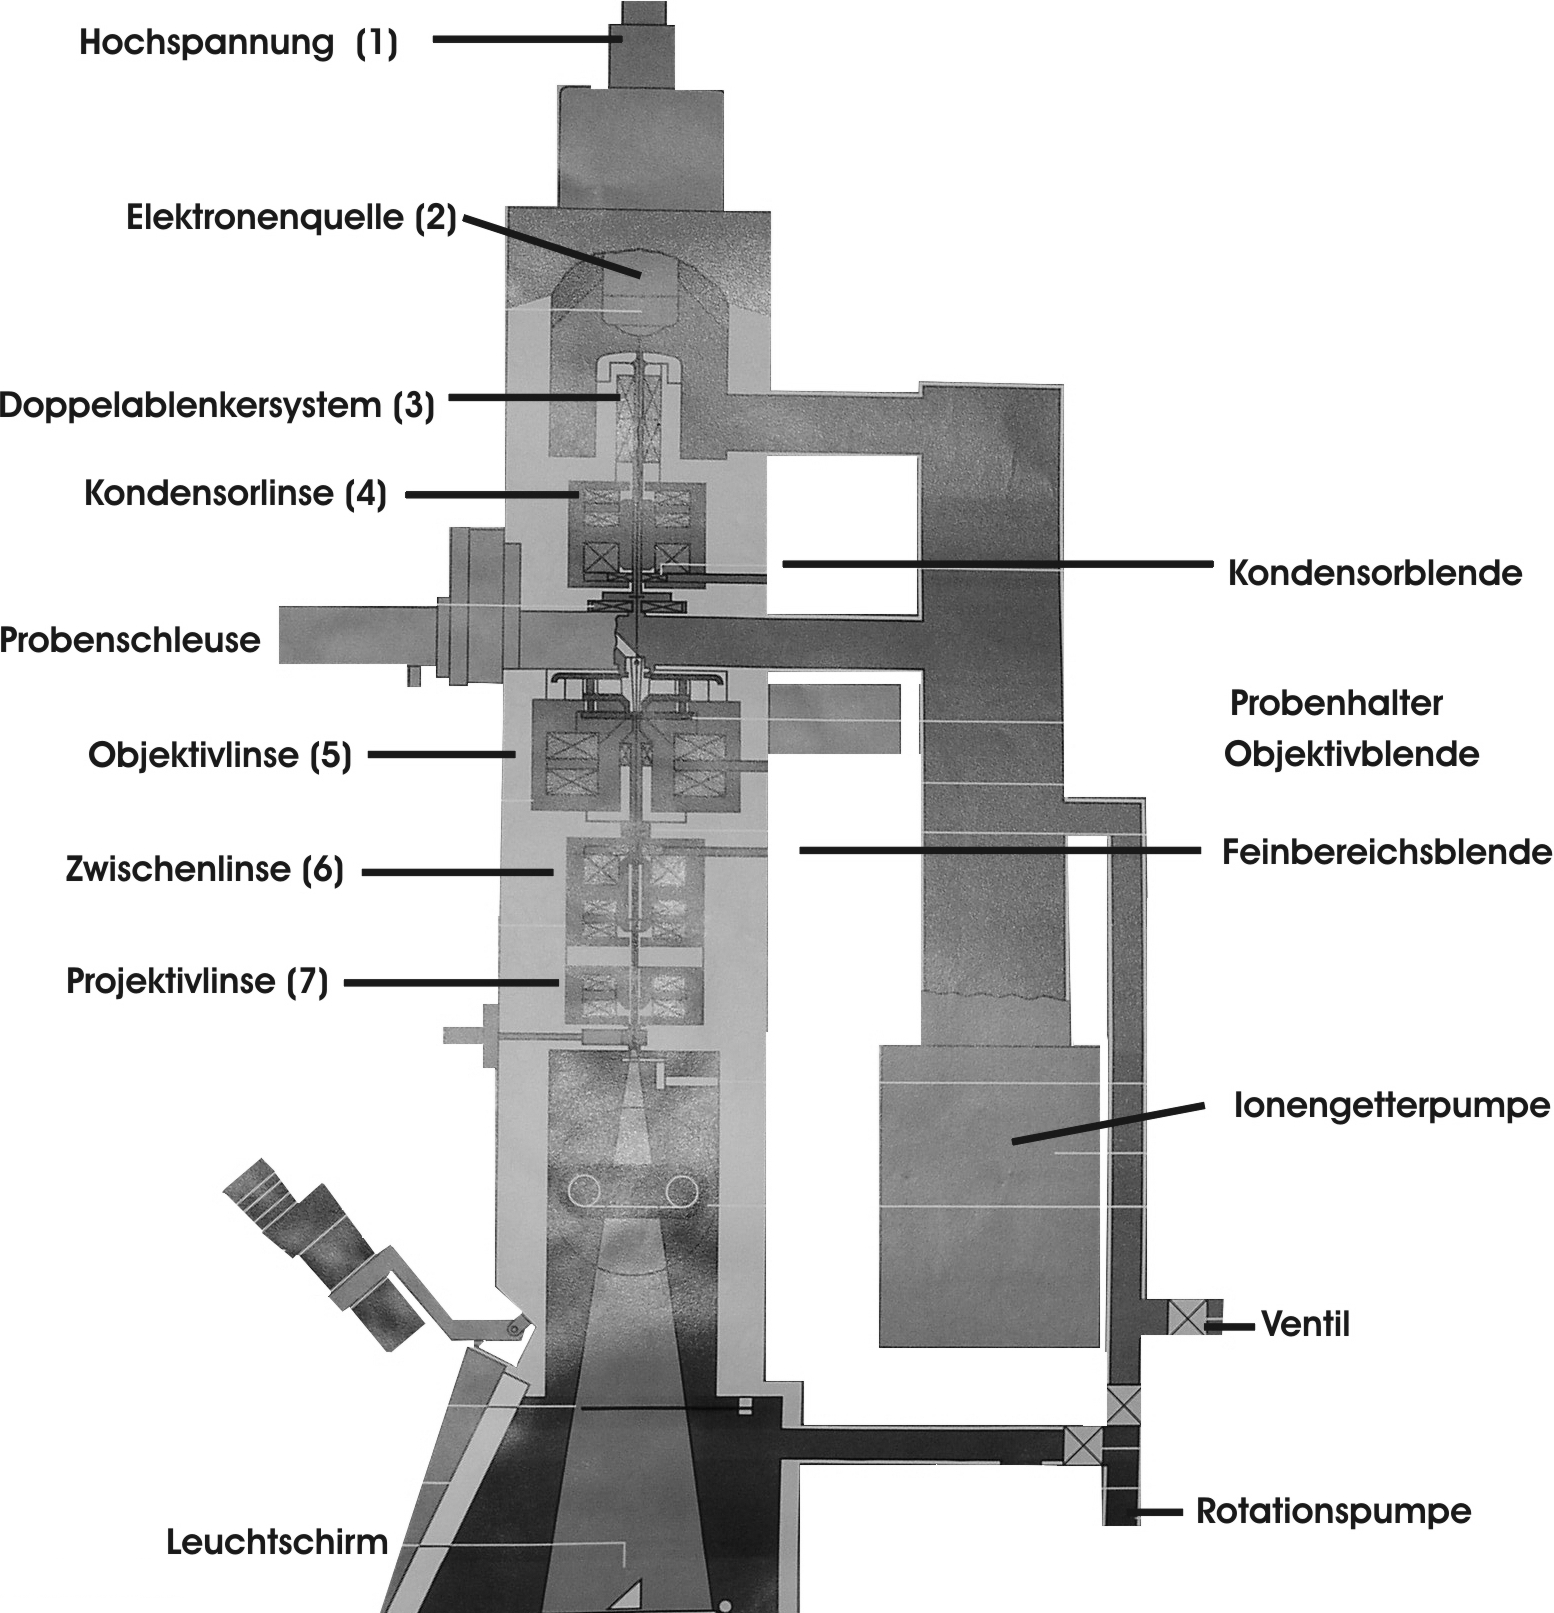
\includegraphics[width=0.7\textwidth]{Zeiss_TEM109.png}
	\caption{Querschnitt eines TEM (Zeiss TEM109) \cite{lit:tueb}}
	\label{fig:setup}
	\vspace{-4em}
\end{figure}


\subsubsection{Unter-, Über-, Fokus}
Liegt die Probe exakt im Fokus der Objektivlinse, so wird sie ohne Interferenzeffekte abgebildet (Abb. \ref{fig:Fokus}). Eine Abweichung von dieser Einstellung wird  als Defokus bezeichnet und führt zu Fresnelsäumen im Bild: Bedingt durch Interferenz bilden sich an Kanten eine Streifenschar aus abwechselnd hellen und dunklen Bereichen.

Wird die Objektivlinse stärker angeregt, so verringert sich die Brennweite und das Objekt liegt unterhalb der Fokusebene. Diese Form der Defokussierung wird als Unterfokus bezeichnet und zeigt sich im Bild durch einen hellen ersten Saum am Rand der Probe  (Abb. \ref{fig:Unter}). Analog spricht man bei positivem Defokus von Überfokus und erkennt dies daran, dass der erste Fresnelsaum dunkel ist  (Abb. \ref{fig:Ueber}).
\begin{figure}[p]
	\vspace{-1.5em}
	\centering
	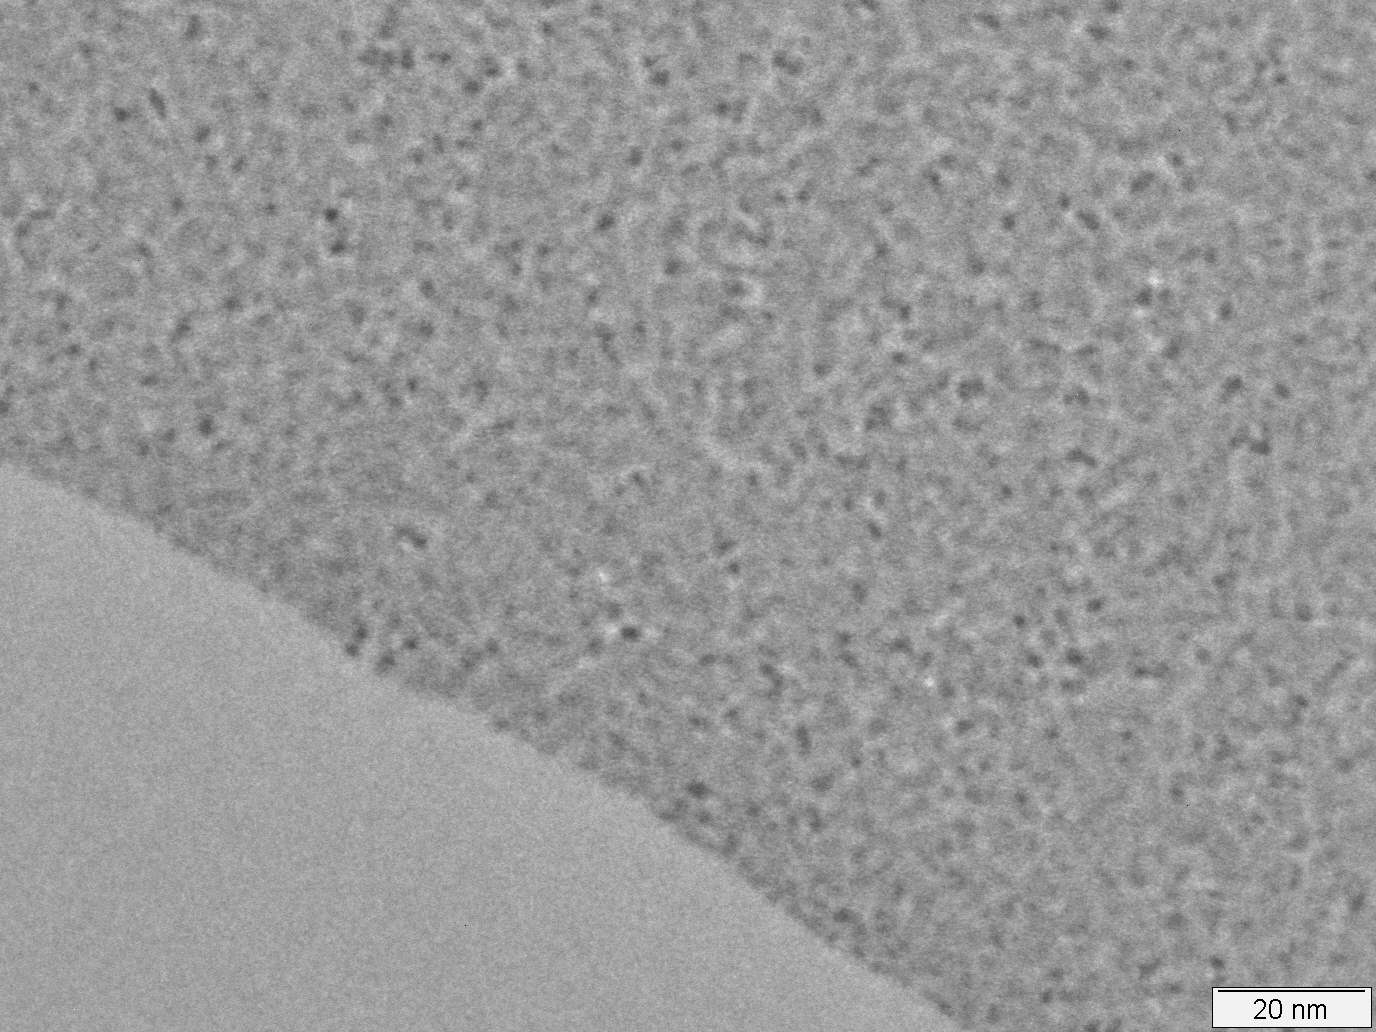
\includegraphics[width=0.68\textwidth]{data/Im_1.jpg}
	\vspace{-1.5ex}
	\caption{Rand der Probe im Fokus, keine Fresnelstreifen}			\label{fig:Fokus}
	\vspace{-1em}
\end{figure}

\begin{figure}[p]
	\centering
	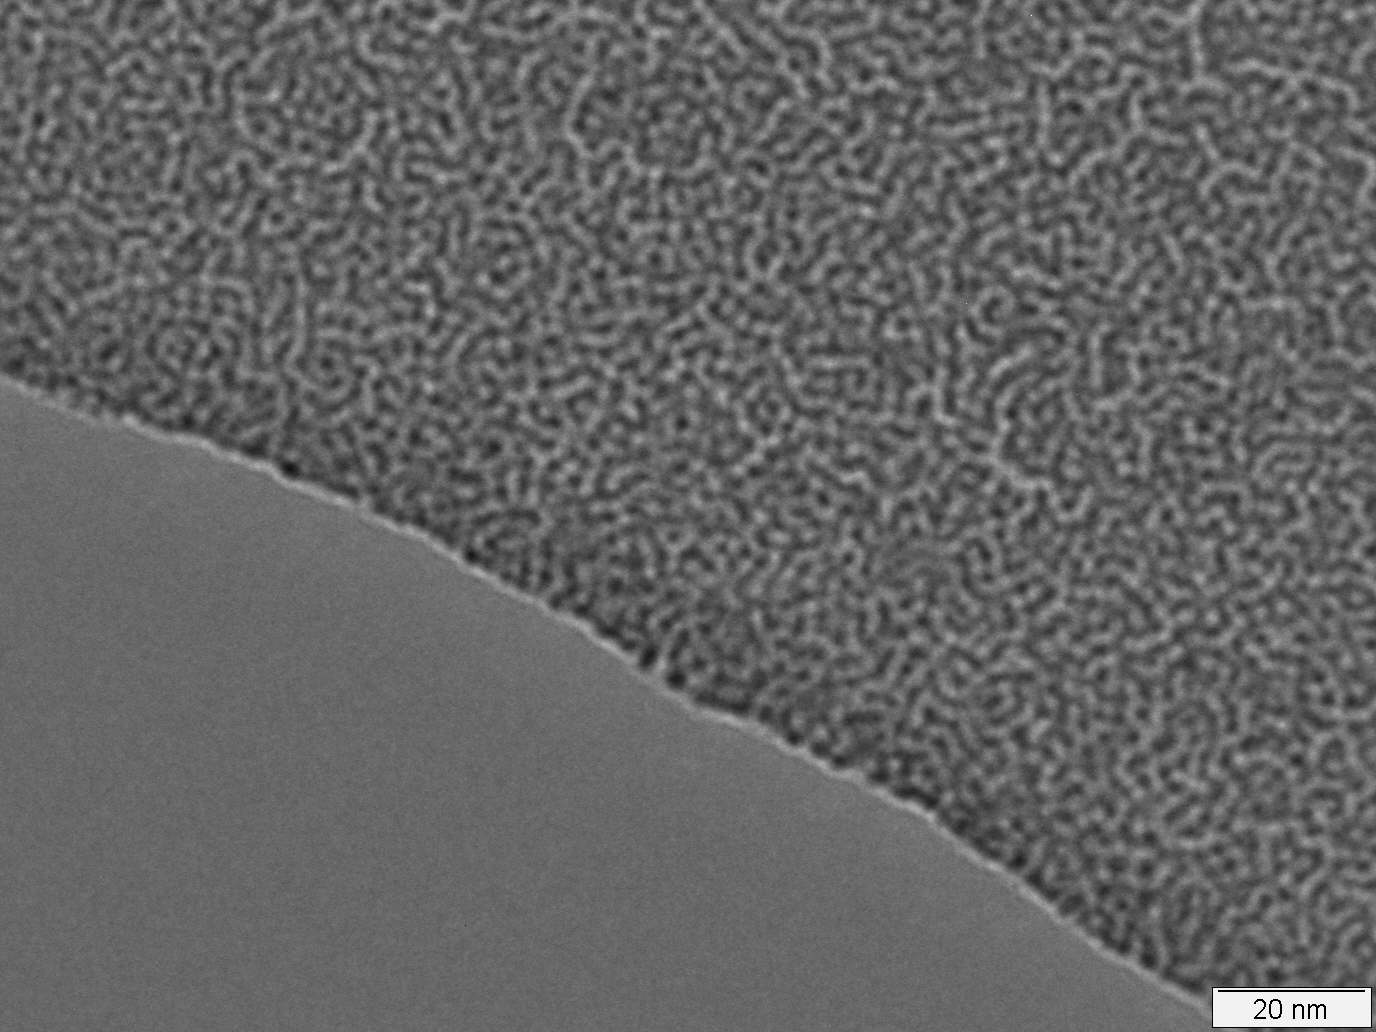
\includegraphics[width=0.68\textwidth]{data/Im_3.jpg}
	\vspace{-1.5ex}
	\caption{Rand der Probe im Unterfokus, erster Fresnelsaum hell}		\label{fig:Unter}
	\vspace{-1em}
\end{figure}

\begin{figure}[p]
	\centering
	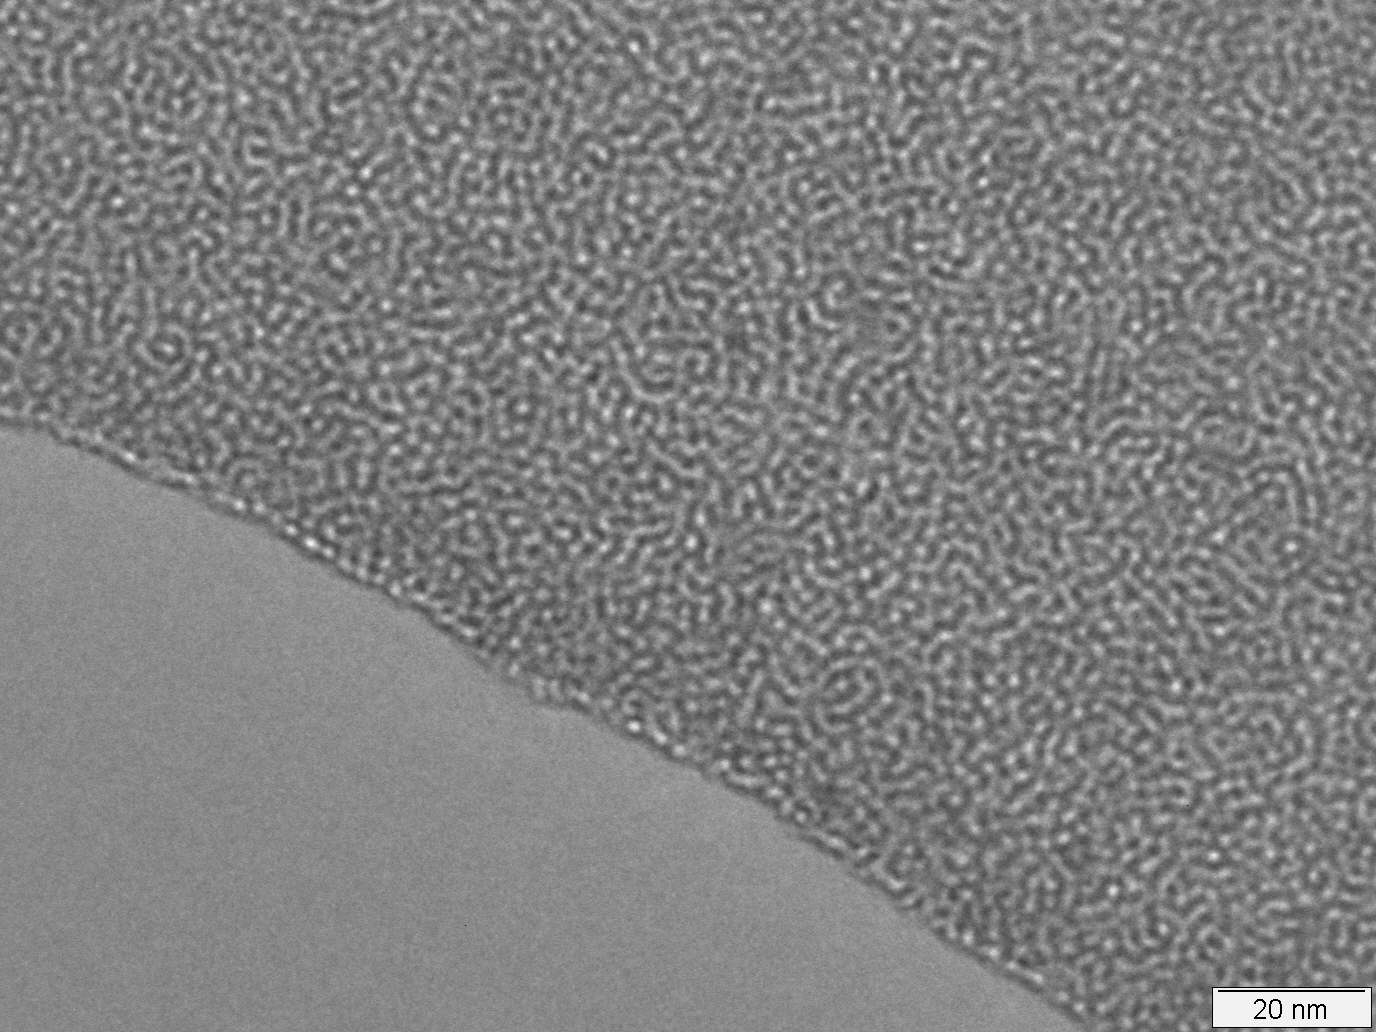
\includegraphics[width=0.68\textwidth]{data/Im_2.jpg}
	\vspace{-1.5ex}
	\caption{Rand der Probe im Überfokus, erster Fresnelsaum dunkel}	\label{fig:Ueber}
	\vspace{-9em}
\end{figure}

\subsubsection{Diffraktogramm und Beugungsbild}
Das Diffraktogramm ist die 2D-Fouriertransformation der Abbildung. Da die Qualität eines solchen errechneten Beugungsbildes geringer ist als eine Aufnahme im Beugungsmodus, wird in diesem Protokoll auf die Wiedergabe von Diffraktogrammen verzichtet. Aus einer TEM-Aufnahme kann z.B. mit der Software ImageJ \cite{lit:ImageJ} das Diffraktogramm auch nachträglich berechnet werden.

% Diffraktogramme nicht auf USB Stick dabei: freies Programm ImageJ, wahrscheinlich auch matlab (2D fft)

Normalerweise zeigt sich im Diffraktogramm ein dunkler Ring, welcher zur Einstellung der Stigmatoren genutzt wird: Zweizähliger Astigmatismus führt zur Verzerrung dieses Rings zu einer Ellipse, bei korrekter Abstimmung der Spannungen an den Multipolen erhält man wieder einen Kreis.

Da die untersuchten Edelmetall-Partikel zufällig orientiert sind, erhalten wir im Beugungsbild Ringe (siehe Abb. \ref{fig:Edel}) anstelle von scharfen Reflexen: Für jeden Azimutwinkel finden sich entsprechend orientierte Partikel, sodass die Bragg-Bedingung erfüllt wird.

Die monokristalline \textsf{Si}-Probe ergibt erwartungsgemäß punktförmige Beugungsreflexe (Abb. \ref{fig:Si}).

\subsubsection{Hellfeld \& Dunkelfeld}
Alle Partikel der Probe tragen zum Hauptstrahl bei, somit sieht man trotz Abblendung aller höheren Ordnungen im Hellfeld-Modus die gesamte Probe (Abb. \ref{fig:TEM_Hell}). Für das Dunkelfeld wählt man mit der Blende jedoch nur einen Ausschnitt des ersten Beugungsringes, im Bild leuchten nur die Partikel mit diesem Azimutwinkel auf (Abb. \ref{fig:TEM_Dunkel}).

\begin{figure}[p]
	\centering
	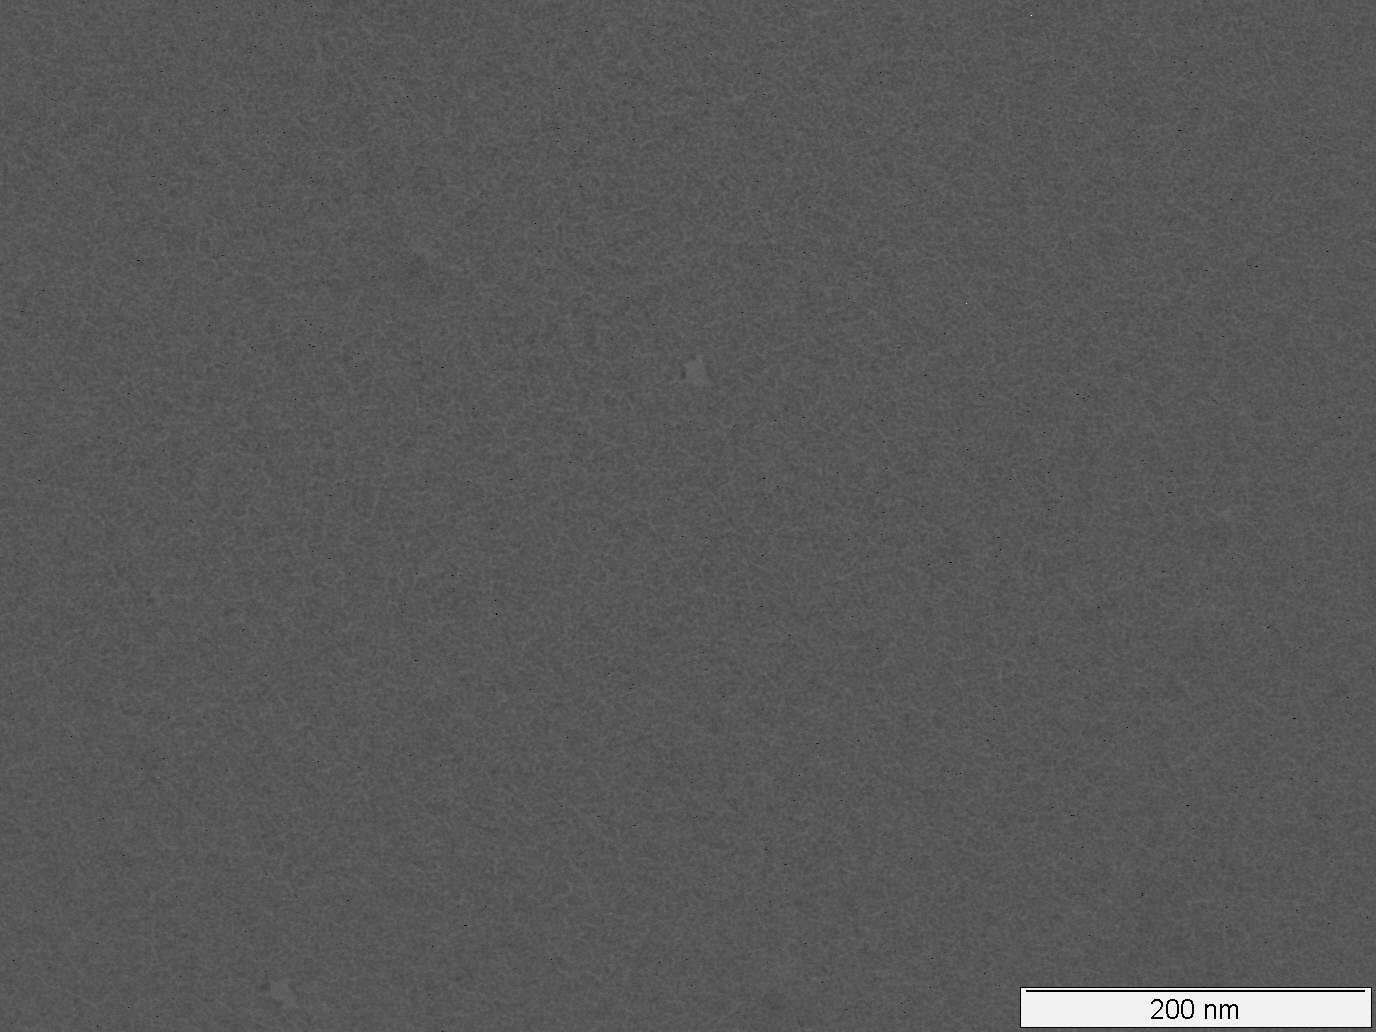
\includegraphics[width=0.9\textwidth]{data/Im_11.jpg}
	\caption{Hellfeld-Bild der Probe, alle Partikel sichtbar}					\label{fig:TEM_Hell}
\end{figure}

\begin{figure}[p]
	\centering
	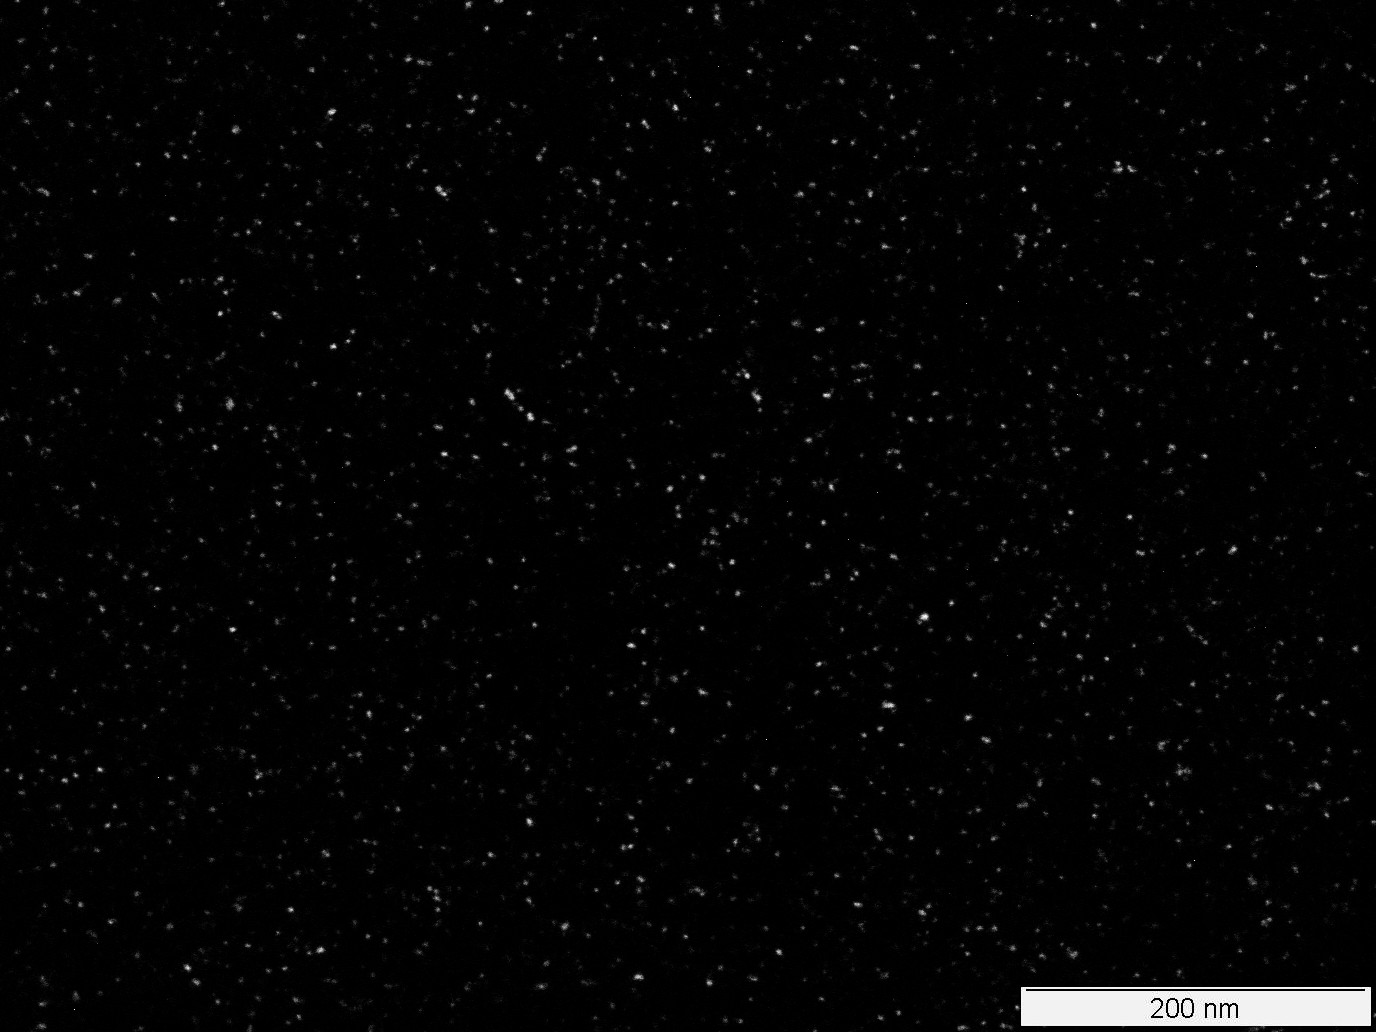
\includegraphics[width=0.9\textwidth]{data/Im_14b.jpg}
	\caption{Dunkelfeld-Bild der Probe, nur korrekt orientierte Partikel sichtbar}	\label{fig:TEM_Dunkel}
	\vspace{-3em}
\end{figure}




\subsubsection{Zulässige Reflexe}
Die Reflexe welcher Ebenen (h\,k\,l) sind im Beugungsbild beobachtbar?

Aus Abb. \ref{fig:laue_bedingung} geht hervor, dass die Laue-Bedingung für alle betrachteten Reflexe näherungsweise erfüllt ist und somit nicht weiter berücksichtigt werden muss.

Es entfallen jedoch alle Reflexe, für die der Strukturfaktor der Basis 0 wird, da sich in diesem Fall die Teilwellen unterschiedlicher Netzebenen aufheben. Sei $f$ der atomare Streufaktor des Elements, dann gilt für fcc-Gitter:
\begin{equation}
S_{hkl}^{fcc} = f \cdt\! \left[1 + i^{2(k+l)} +  i^{2(h+l)} +  i^{2(h+k)} \right] =
\begin{cases}
4 f	& h\,k\,l \text{ gerade} \lor h\,k\,l \text{ ungerade}\\
0	& \text{sonst}
\end{cases}
\end{equation}

Das Diamant-Kristallgitter des Siliziums besteht aus zwei um $(\frac14 \frac14 \frac14)$ verschobenen fcc-Gittern, was die zulässigen Reflexe nochmals einschränkt:
\begin{equation}
S_{hkl}^\mathsf{Si} =  S_{hkl}^{fcc} \cdt \left[1 + i^{h+k+l} \right] \somit \tfrac14 ~ (h+k+l) \in \mathds{N}
\end{equation}

Zudem ist der \textsf{Si}-Kristall entlang der 110 Achse orientiert, folglich tritt nur an zu dieser senkrechten Ebenen Bragg-Reflexion auf:
\begin{equation}
(h\,k\,l) \perp [1\,1\,0]		\quad\iff\quad	1 \cdt h + 1 \cdt k + 0 \cdt l = 0
\end{equation}

Aus diesem Grund erwarten wir folgende Reflexe für die beiden Proben, wobei Vorzeichen vernachlässigt wurden:

\begin{table}[h]
\centering
\caption{Zulässige Reflexe}
\begin{tabular}{*{13}c}
	\toprule
	Metall-Pulver		& 111	& 002	& 220	& 113	& 222	& 004	& 331	& 224	& 115	& 333	& 440	& \dots	\\
	\textsf{Si}-Kristall	& 111	&		& 220	& 113	&		& 004	& 331	& 224	& 115	& 333	& 440	&  \dots	\\
	\midrule
	$h^2 + k^2 + l^2$	& 3		& 4		& 8		& 11		& 12		& 16		& 19		& 24		& 27		& 27		& 32 \\
	\bottomrule
\end{tabular}
\end{table}

\newpage
\subsubsection{Bestimmung der Gitterkonstante}
Für sämtliche Beugungsbilder wurde das TEM auf 340\,mm Kameraabstand (entsprechend 30000\,facher Vergrößerung) bzw. 300\,mm Schirmabstand (26500x Vergrößerung) eingestellt.

Neben Abbildung \ref{fig:Edel} und \ref{fig:Si} wurde jeweils noch eine Aufnahme bei schwächerer Belichtung erstellt, da auf diesen die hellsten Beugungsordnungen schärfer sind. Die Abstände $\kappa$ in Pixeln der verschiedenen Beugungsordnungen vom Ursprung wurden aus den Ringdurchmessern bzw. den Abständen gegenüberliegender Punkte ermittelt, da das Halbieren der Längen die Ablesefehler verringert.

Der Fehler $\Delta \kappa$ variierte zwischen $\pm 2$ und $\pm 4$ Pixeln, je nach Breite des gemessenen Peaks bzw. Rings. Aus diesem erhielten wir mit Gleichungen \eqref{eq:scale} und \eqref{eq:da} die Genauigkeit des Ergebnisses.

Mithilfe der bekannten Gitterkonstante $a_\mathsf{Si} = 543,102\,\pico\metre$ \cite{lit:nist} lässt sich der Maßstab des Beugungsbildes ermitteln:
\begin{equation}
\kappa ~\propto~ \frac{1}{d_{hkl}}		\somit c ~:=~ \kappa \cdt d_{hkl}
\label{eq:scale}
\end{equation}

Wie in Tabelle \ref{tab:Si} ersichtlich, konnten wir auch die eigentlich in der Diamant-Konfiguration fehlenden Reflexe bei 002 und 222 messen. Dies wäre nur bei unterschiedlichen Atomen in der zweiatomigen Basis zu erwarten, was bei Silizium aber nicht der Fall ist.

\begin{table}[p]
\centering
\caption{Beugungsreflexe für den 110 orientierten \textsf{Si}-Kristall}	\label{tab:Si}
\begin{tabular}{*4c}
	\toprule
	Anzahl $n$		& $h\,k\,l$		& $\kappa$ in px	& $c$ in pm$\cdt$px	\\
	\midrule
	4	& 111		& 142 $\pm$ 2	& 44500 $\pm$ 700	\\
	2	& 002		& 164 $\pm$ 4	& 44400 $\pm$ 1100	\\
	2	& 220		& 231 $\pm$ 2	& 44300 $\pm$ 400	\\
	4	& 113		& 271 $\pm$ 2	& 44400 $\pm$ 400	\\
	4	& 222		& 283 $\pm$ 2	& 44300 $\pm$ 400	\\
	2	& 004		& 328 $\pm$ 2	& 44530 $\pm$ 280	\\
	4	& 331		& 355 $\pm$ 2	& 44170 $\pm$ 250	\\
	4	& 224		& 400 $\pm$ 2	& 44340 $\pm$ 230	\\
	2	& 115 \& 333	& 422 $\pm$ 2	& 44110 $\pm$ 210	\\
	2	& 440		& 460 $\pm$ 2	& 44160 $\pm$ 200	\\
	\midrule
		&			&			& 44320 $\pm$ 200	\\
	\bottomrule
\end{tabular}
\end{table}

Abschließend ermitteln wir die Gitterkonstante der unbekannten Probe:
\begin{align}
a^*		~&=~ \frac{c \cdt \sqrt{h^2 + k^2 + l^2}}{\kappa}	\\
\Delta a^*	~&=~ \frac{\sqrt{h^2 + k^2 + l^2}}{\kappa^2} \cdt \sqrt{ (\kappa ~ \Delta c)^2 + (c ~ \Delta \kappa)^2}
\label{eq:da}
\end{align}

\begin{table}[p]
\centering
\caption{Beugungsreflexe für das Metall-Pulver}	\label{tab:Edel}
\begin{tabular}{*3c}
	\toprule
	$h\,k\,l$	& $\kappa$ in px	& $a^*$ in pm	\\
	\midrule
	111		& 184 $\pm$ 3		& 417 $\pm$ 8		\\
	002		& 211 $\pm$ 3		& 420 $\pm$ 7		\\
	220		& 298 $\pm$ 3		& 421 $\pm$ 5		\\
	113		& 351 $\pm$ 3		& 419 $\pm$ 5		\\
	331		& 465 $\pm$ 3		& 416 $\pm$ 4		\\
	135		& 627 $\pm$ 3		& 418,2 $\pm$ 2,8		\\
	\midrule
			&				& 418,5 $\pm$ 2,8	\\
	\bottomrule
\end{tabular}
\end{table}

Wir erhalten eine Gitterkonstante von $a^* = 418,5 \pm 2,8$\,pm, welche leicht oberhalb der Werte für Edelmetalle liegt. Unser Wert kommt $a_\mathsf{Ag} = 408,53\,\pico\metre$ und $a_\mathsf{Au} = 407,82\,\pico\metre$ recht nahe, weshalb es sich um eines dieser beiden Edelmetale handeln dürfte \cite{lit:elements}.

Da es sich um Nanopartikel handelt, könnten diese auch durch Verspannungen eine leicht andere Gitterkonstante aufweisen als üblich -- allerdings ist dieser Effekt meist entgegengesetzt, da die Oberflächenspannung die Partikel zusammendrückt.



\begin{figure}[p]
	\centering
	\begingroup
	\setlength{\unitlength}{0.9\textwidth}
	\begin{picture}(1,0.75)
		\put(0,0){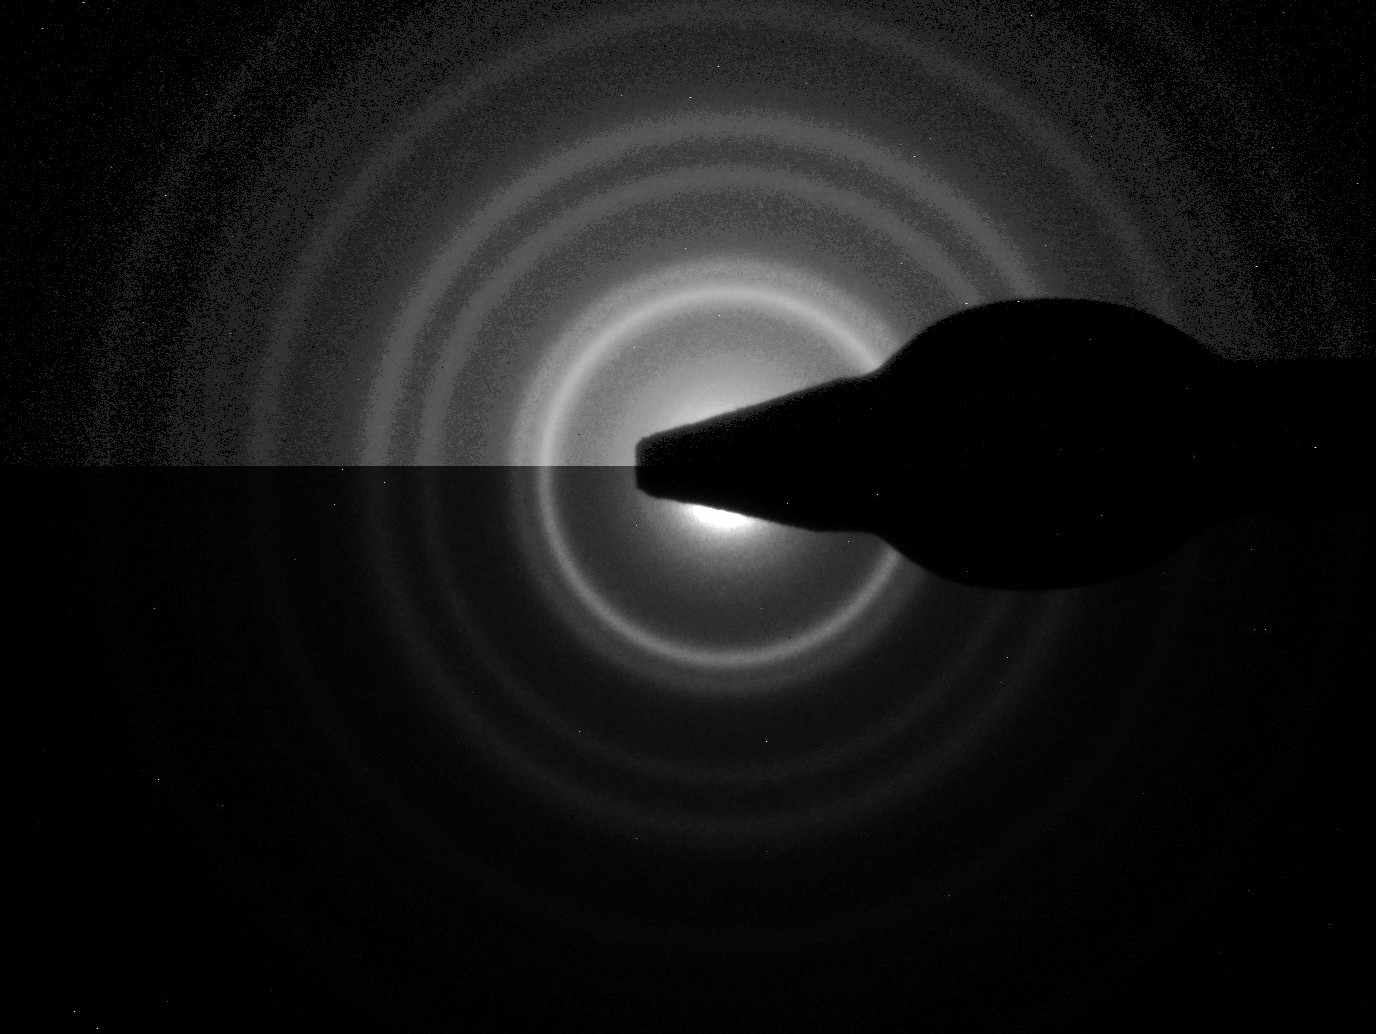
\includegraphics[width=\unitlength]{data/Im_10c.jpg}}
		\color{yellow!60!orange}
		\put(0.5	,0.28   ){111}
		\put(0.5	,0.23   ){002}
		\put(0.5	,0.18   ){220}
		\put(0.5	,0.135 ){113}
		\put(0.17	,0.39  ){331}
		\put(0.05	,0.39  ){135}
	\end{picture}
	\endgroup
	\caption{Beugungsbild des Edelmetall-Pulvers}				\label{fig:Edel}
\end{figure}

\begin{figure}[p]
	\centering
	\begingroup
	\setlength{\unitlength}{0.9\textwidth}
	\begin{picture}(1,0.75)
		\put(0,0){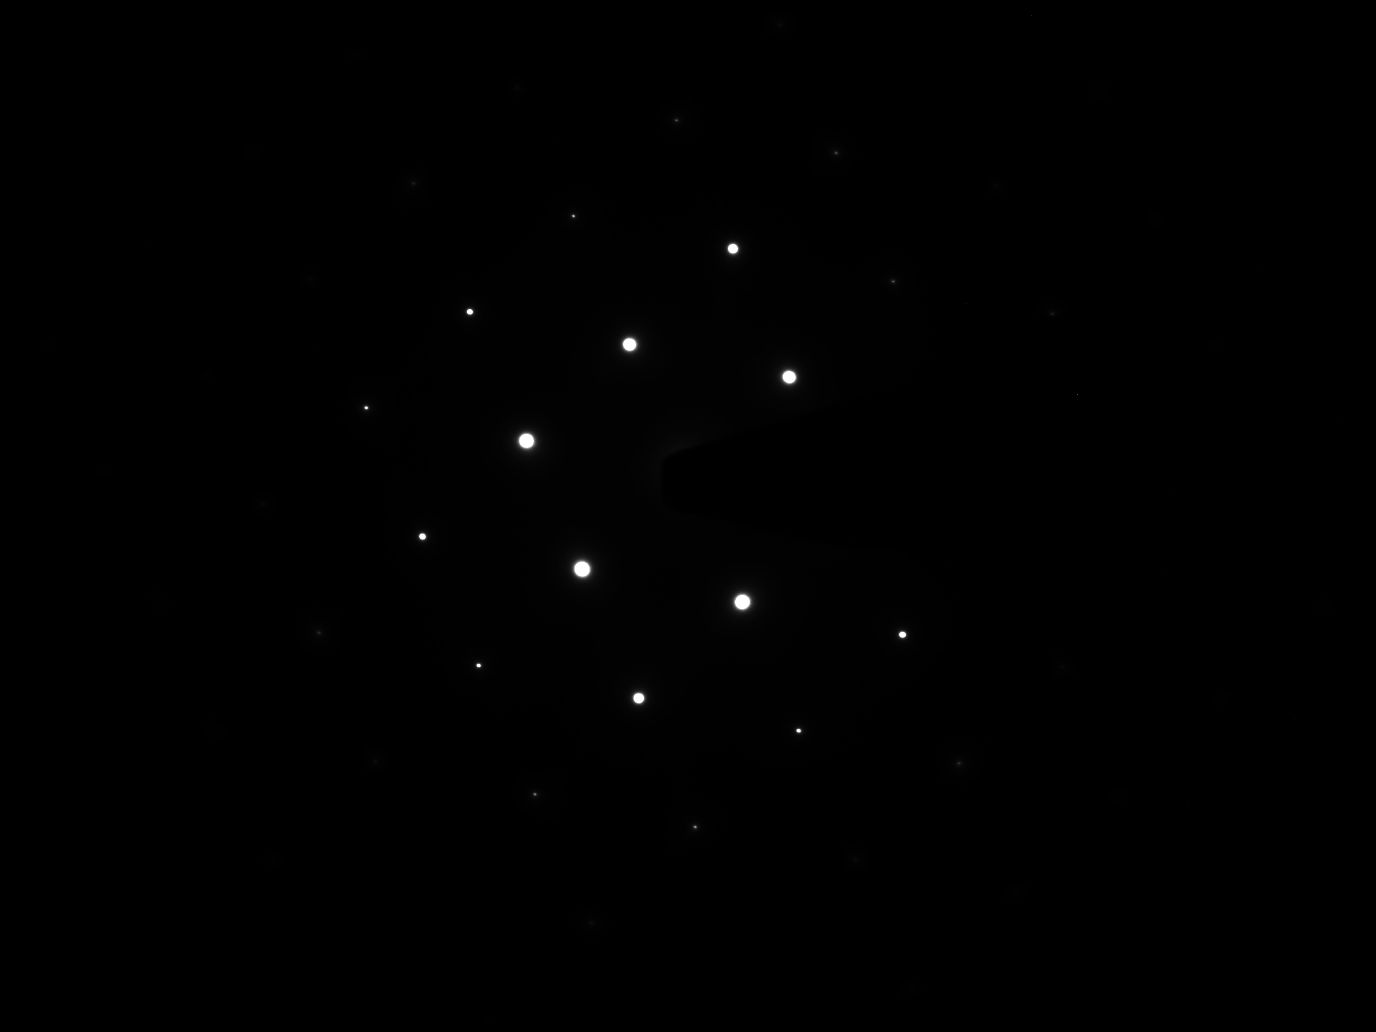
\includegraphics[width=\unitlength]{data/Im_22.jpg}}
		\color{yellow!60!orange}
		\put(0.36	,0.395	){002}
		\put(0.4	,0.3		){111}
		\put(0.52	,0.275	){111}
		\put(0.435	,0.46		){111}
		\put(0.555	,0.44		){111}
		\put(0.443	,0.208	){220}
		\put(0.51	,0.535	){220}
		\put(0.245	,0.42		){004}
		\put(0.285	,0.325	){113}
		\put(0.32	,0.49		){113}
		\put(0.635	,0.255	){113}
		\put(0.33	,0.235	){222}
		\put(0.395	,0.563	){222}
		\put(0.628	,0.517	){222}
		\put(0.56	,0.19		){222}
		\put(0.485	,0.115	){331}
		\put(0.47	,0.633	){331}
		\put(0.587	,0.61		){331}
		\put(0.367	,0.14		){331}
		\put(0.406	,0.05		){440}
		\put(0.543	,0.702	){440}
		\put(0.212	,0.26		){224}
		\put(0.675	,0.165	){224}
		\put(0.28	,0.586	){224}
		\put(0.745	,0.492	){224}
		\put(0.6	,0.095	){333}
		\put(0.25	,0.167	){333}
	\end{picture}
	\endgroup
	\caption{Beugungsbild des Silizium-Kristalls (110 Orientierung)}	\label{fig:Si}
	\vspace{-5em}
\end{figure}


% I = imread('Im22.png');
% I2 = im2double(I);



% Edelmetall-Probe:
% High resolution (mehrere bilder mit Netz ebenen)
% Im_5, Im_6
% Meist nur eine Schar Netzebenen sichtbar (anstatt kariert) da die meisten Körner nicht in der fokusebene orientiert sind und somit nur eine Achse passt




% Si
% convergent beam (Kreise mit gebogenem Linien, geben Aufschluss über dicke der probe)
% Im_20
